% !TeX program = pdflatex
% !BIB program = biber
% ==============================================================================
% Modelo de Trabalho de Conclusão de Curso (TCC) do tipo CIENTÍFICO
% Ciência da Computação e Engenharia de Computação | DCE/Ceunes/Ufes
%
% Normas: ABNT NBR 14724:2024 (trabalhos acadêmicos), NBR 10520:2023
% (citações), NBR 6023 (referências), NBR 6024:2012 (numeração progressiva),
% NBR 6027:2012 (sumário) e NBR 6028:2021 (resumo).
%
% Adaptado do modelo do DI/CT/Ufes (Prof. Vítor E. Silva Souza), baseado no
% abnTeX2. Distribuído sob a LaTeX Project Public License 1.3c.
%
% Comece pelo arquivo cientifico/dados.tex. O texto de cada capítulo traz um
% exemplo fictício (uma heurística para o problema da mochila multidimensional)
% e caixas de orientação que explicam o que escrever em cada parte.
% ==============================================================================

\documentclass[
  12pt,           % tamanho da fonte (NBR 14724 recomenda 12)
  a4paper,        % papel A4
  oneside,        % entrega em PDF: cada seção primária começa em nova página
  openany,
  chapter=TITLE,  % títulos das seções primárias em caixa alta
  english,        % idioma adicional (abstract)
  brazil,         % idioma principal (deve ser o último)
]{abntex2}

% ------------------------------------------------------------------------------
% Chaves de controle
% ------------------------------------------------------------------------------
% Caixas de orientação: troque para \mostrarinstrucoesfalse quando não
% precisar mais delas (obrigatório na versão entregue à banca).
\newif\ifmostrarinstrucoes
\mostrarinstrucoestrue

% Notas de revisão \notaaluno{...} e \notaorientador{...}.
\newif\ifmostrarnotas
\mostrarnotastrue

% ------------------------------------------------------------------------------
% Preâmbulo
% ------------------------------------------------------------------------------
% ==============================================================================
% config/pacotes.tex
% Pacotes usados pelo modelo. Em geral, não é preciso alterar este arquivo.
% Se precisar de um pacote novo, acrescente-o ao final, na área indicada.
% ==============================================================================

% ------------------------------------------------------------------------------
% Fontes
% ------------------------------------------------------------------------------
% O modelo compila com pdfLaTeX (padrão), XeLaTeX ou LuaLaTeX. O pacote iftex
% identifica o compilador e carrega apenas o que cada um precisa.
\usepackage{iftex}
\ifPDFTeX
  \usepackage[T1]{fontenc}
  \usepackage{lmodern}   % Latin Modern Mono para códigos (texto e títulos usam Libertine)
\fi

% Linux Libertine (texto) e Linux Biolinum (sem serifa). A opção mono=false
% mantém a fonte monoespaçada padrão, mais legível em listagens de código.
\usepackage[mono=false]{libertine}

% Matemática com o mesmo desenho da Libertine. O libertinust1math já define os
% símbolos do amssymb, por isso este último não deve ser carregado.
\usepackage{amsmath}
\usepackage{libertinust1math}

% Vírgula decimal em modo matemático sem espaço extra: $3,14$.
\usepackage{icomma}

% Ajustes finos de justificação e hifenização.
\usepackage{microtype}

% Recuo também no primeiro parágrafo de cada seção.
\usepackage{indentfirst}

% ------------------------------------------------------------------------------
% Cores, figuras e gráficos
% ------------------------------------------------------------------------------
\usepackage[dvipsnames,table]{xcolor}
\usepackage{graphicx}
\usepackage{subcaption}
\usepackage{pgfplots}
\pgfplotsset{compat=1.18}
\usetikzlibrary{positioning,arrows.meta,shapes.multipart,shapes.geometric,fit,calc,backgrounds}

% ------------------------------------------------------------------------------
% Tabelas
% ------------------------------------------------------------------------------
\usepackage{array}
\usepackage{booktabs}
\usepackage{multirow}
\usepackage{tabularx}
\usepackage{longtable}

% ------------------------------------------------------------------------------
% Códigos e algoritmos
% ------------------------------------------------------------------------------
\usepackage{listings}
\usepackage{algpseudocode}

% ------------------------------------------------------------------------------
% Caixas de orientação e exemplos (podem ser desligadas no arquivo principal)
% ------------------------------------------------------------------------------
\usepackage{comment}
\usepackage[most]{tcolorbox}

% ------------------------------------------------------------------------------
% Citações e referências (ABNT NBR 10520:2023 e NBR 6023)
% ------------------------------------------------------------------------------
% Requer biblatex-abnt 4.0 ou mais recente (TeX Live 2024 em diante) e o Biber
% como processador de bibliografia.
\usepackage[autostyle]{csquotes}
\usepackage[style=abnt, backend=biber]{biblatex}

% ------------------------------------------------------------------------------
% Referências cruzadas e siglas
% ------------------------------------------------------------------------------
\usepackage[nameinlink,noabbrev]{cleveref}
\usepackage{acro}

% ------------------------------------------------------------------------------
% Notas de revisão entre aluno e orientador
% ------------------------------------------------------------------------------
\ifmostrarnotas
  \usepackage[colorinlistoftodos,textsize=footnotesize]{todonotes}
\else
  \usepackage[disable]{todonotes}
\fi

\usepackage{xspace}

% ------------------------------------------------------------------------------
% Pacotes adicionais do aluno
% ------------------------------------------------------------------------------
% \usepackage{...}

% ==============================================================================
% config/estilo.tex
% Aparência do documento: títulos, legendas, ilustrações, códigos, referências
% cruzadas, siglas e caixas de orientação. Em geral, não é preciso alterar.
% ==============================================================================

% ------------------------------------------------------------------------------
% Termo usado para as divisões principais do texto
% ------------------------------------------------------------------------------
% A NBR 14724:2024 (item 4.2.2) determina que o trabalho seja organizado em
% seções, e não em capítulos. O padrão abaixo segue as regras de TCC do curso.
% Para adotar a terminologia da norma, troque por {Seção} e {Seções} e revise
% os artigos no texto ("o Capítulo 2" passa a ser "a Seção 2").
\newcommand{\termocap}{Capítulo}
\newcommand{\termocaps}{Capítulos}

% ------------------------------------------------------------------------------
% Parágrafos e títulos
% ------------------------------------------------------------------------------
\setlength{\parindent}{1.25cm}

% Destaque gráfico progressivo das seções (NBR 6024). O caixa alta das seções
% primárias vem da opção chapter=TITLE da classe.
\renewcommand{\ABNTEXchapterfont}{\normalfont\bfseries}
\renewcommand{\ABNTEXchapterfontsize}{\large}
\renewcommand{\ABNTEXsectionfont}{\normalfont\bfseries}
\renewcommand{\ABNTEXsectionfontsize}{\normalsize}
\renewcommand{\ABNTEXsubsectionfont}{\normalfont\bfseries\itshape}
\renewcommand{\ABNTEXsubsectionfontsize}{\normalsize}
\renewcommand{\ABNTEXsubsubsectionfont}{\normalfont\itshape}
\renewcommand{\ABNTEXsubsubsectionfontsize}{\normalsize}

% ------------------------------------------------------------------------------
% Legendas e fontes das ilustrações e tabelas
% ------------------------------------------------------------------------------
% A NBR 14724 pede fonte menor e uniforme para legendas, fontes, notas e
% citações longas. O abnTeX2 usa \footnotesize para \fonte e citações longas.
\captionsetup{font=footnotesize}
\captionsetup[sub]{font=footnotesize}

% Texto padrão para material elaborado pelo próprio autor (NBR 14724:2024).
\newcommand{\fonteautor}{\fonte{Elaborado pelo próprio autor.}}

% Posição padrão dos objetos flutuantes.
\setfloatlocations{figure}{htbp}
\setfloatlocations{table}{htbp}

% ------------------------------------------------------------------------------
% Novos tipos de ilustração: Quadro, Código e Algoritmo
% ------------------------------------------------------------------------------
% Quadro: informação textual organizada em linhas e colunas, com bordas
% fechadas. Tabela: dados numéricos, sem bordas laterais (normas do IBGE).
\newcommand{\quadroname}{Quadro}
\newcommand{\listofquadrosname}{Lista de quadros}
\newfloat{quadro}{loq}{\quadroname}
\newlistof{listofquadros}{loq}{\listofquadrosname}
\newlistentry{quadro}{loq}{0}
\setfloatlocations{quadro}{htbp}
\renewcommand{\cftquadroname}{\quadroname\space}
\renewcommand*{\cftquadroaftersnum}{\hfill\textendash\hfill}

\newcommand{\codigoname}{Código}
\newcommand{\listofcodigosname}{Lista de códigos}
\newfloat{codigo}{lcod}{\codigoname}
\newlistof{listofcodigos}{lcod}{\listofcodigosname}
\newlistentry{codigo}{lcod}{0}
\setfloatlocations{codigo}{htbp}
\renewcommand{\cftcodigoname}{\codigoname\space}
\renewcommand*{\cftcodigoaftersnum}{\hfill\textendash\hfill}

\newcommand{\algoritmoname}{Algoritmo}
\newcommand{\listofalgoritmosname}{Lista de algoritmos}
\newfloat{algoritmo}{lalg}{\algoritmoname}
\newlistof{listofalgoritmos}{lalg}{\listofalgoritmosname}
\newlistentry{algoritmo}{lalg}{0}
\setfloatlocations{algoritmo}{htbp}
\renewcommand{\cftalgoritmoname}{\algoritmoname\space}
\renewcommand*{\cftalgoritmoaftersnum}{\hfill\textendash\hfill}

% Largura reservada para o rótulo ("Quadro 10", "Código 10" etc.) nas listas.
\setlength{\cftquadronumwidth}{2.5em}
\setlength{\cftcodigonumwidth}{2.5em}
\setlength{\cftalgoritmonumwidth}{2.5em}

% ------------------------------------------------------------------------------
% Códigos (pacote listings)
% ------------------------------------------------------------------------------
\definecolor{codigofundo}{gray}{0.96}
\definecolor{codigocomentario}{gray}{0.40}
\definecolor{codigonumero}{gray}{0.55}

\lstset{
  basicstyle=\ttfamily\footnotesize\linespread{1}\selectfont,
  keywordstyle=\bfseries,
  commentstyle=\itshape\color{codigocomentario},
  stringstyle=\color{black},
  numbers=left,
  numberstyle=\tiny\color{codigonumero},
  numbersep=8pt,
  backgroundcolor=\color{codigofundo},
  frame=tb,
  framerule=0.4pt,
  xleftmargin=1.5em,
  breaklines=true,
  breakatwhitespace=true,
  showstringspaces=false,
  tabsize=4,
  columns=fullflexible,
  keepspaces=true,
  upquote=true,
  extendedchars=true,
  inputencoding=utf8,
  % Acentos dentro de códigos e comentários (necessário com pdfLaTeX).
  literate=
    {á}{{\'a}}1 {à}{{\`a}}1 {ã}{{\~a}}1 {â}{{\^a}}1
    {é}{{\'e}}1 {ê}{{\^e}}1 {í}{{\'i}}1
    {ó}{{\'o}}1 {õ}{{\~o}}1 {ô}{{\^o}}1 {ú}{{\'u}}1 {ü}{{\"u}}1
    {ç}{{\c{c}}}1
    {Á}{{\'A}}1 {À}{{\`A}}1 {Ã}{{\~A}}1 {Â}{{\^A}}1
    {É}{{\'E}}1 {Ê}{{\^E}}1 {Í}{{\'I}}1
    {Ó}{{\'O}}1 {Õ}{{\~O}}1 {Ô}{{\^O}}1 {Ú}{{\'U}}1
    {Ç}{{\c{C}}}1
}

% ------------------------------------------------------------------------------
% Algoritmos (pacote algpseudocode) com palavras-chave em português
% ------------------------------------------------------------------------------
\algrenewcommand\algorithmicrequire{\textbf{Entrada:}}
\algrenewcommand\algorithmicensure{\textbf{Saída:}}
\algrenewcommand\algorithmicif{\textbf{se}}
\algrenewcommand\algorithmicthen{\textbf{então}}
\algrenewcommand\algorithmicelse{\textbf{senão}}
\algrenewcommand\algorithmicend{\textbf{fim}}
\algrenewcommand\algorithmicwhile{\textbf{enquanto}}
\algrenewcommand\algorithmicdo{\textbf{faça}}
\algrenewcommand\algorithmicfor{\textbf{para}}
\algrenewcommand\algorithmicforall{\textbf{para todo}}
\algrenewcommand\algorithmicrepeat{\textbf{repita}}
\algrenewcommand\algorithmicuntil{\textbf{até que}}
\algrenewcommand\algorithmicreturn{\textbf{retorne}}
\algrenewcommand\algorithmicfunction{\textbf{função}}
\algrenewcommand\algorithmicprocedure{\textbf{procedimento}}
\algrenewcommand{\algorithmiccomment}[1]{\hfill\(\triangleright\) #1}

% ------------------------------------------------------------------------------
% Gráficos (pgfplots) com vírgula decimal e ponto como separador de milhar
% ------------------------------------------------------------------------------
\pgfplotsset{
  /pgf/number format/.cd, use comma, 1000 sep={.},
}

% ------------------------------------------------------------------------------
% Referências cruzadas (cleveref)
% ------------------------------------------------------------------------------
% Use \cref{rotulo} no meio da frase e \Cref{rotulo} no início. Nos dois casos
% o nome sai com inicial maiúscula ("Figura 3", "Tabela 2"), como pede a norma.
\crefname{chapter}{\termocap}{\termocaps}
\Crefname{chapter}{\termocap}{\termocaps}
\crefname{section}{Seção}{Seções}
\Crefname{section}{Seção}{Seções}
\crefname{subsection}{Seção}{Seções}
\Crefname{subsection}{Seção}{Seções}
\crefname{subsubsection}{Seção}{Seções}
\Crefname{subsubsection}{Seção}{Seções}
\crefname{appendix}{Apêndice}{Apêndices}
\Crefname{appendix}{Apêndice}{Apêndices}
% O abnTeX2 não aciona a detecção de apêndices do cleveref. Dentro dos
% ambientes de apêndices e anexos, os capítulos passam a ser referenciados
% como "Apêndice A" e "Anexo A".
\AtBeginEnvironment{apendicesenv}{\crefalias{chapter}{appendix}}
\AtBeginEnvironment{anexosenv}{\crefalias{chapter}{anexo}}
\crefname{figure}{Figura}{Figuras}
\Crefname{figure}{Figura}{Figuras}
\crefname{subfigure}{Figura}{Figuras}
\Crefname{subfigure}{Figura}{Figuras}
\crefname{table}{Tabela}{Tabelas}
\Crefname{table}{Tabela}{Tabelas}
\crefname{quadro}{Quadro}{Quadros}
\Crefname{quadro}{Quadro}{Quadros}
\crefname{codigo}{Código}{Códigos}
\Crefname{codigo}{Código}{Códigos}
\crefname{algoritmo}{Algoritmo}{Algoritmos}
\Crefname{algoritmo}{Algoritmo}{Algoritmos}
\crefname{equation}{Equação}{Equações}
\Crefname{equation}{Equação}{Equações}
\crefname{page}{página}{páginas}
\Crefname{page}{Página}{Páginas}
\creflabelformat{equation}{(#2#1#3)}
\crefrangelabelformat{equation}{(#3#1#4) a (#5#2#6)}
\newcommand{\crefpairconjunction}{ e }
\newcommand{\crefmiddleconjunction}{, }
\newcommand{\creflastconjunction}{ e }
\newcommand{\crefrangeconjunction}{ a }

% ------------------------------------------------------------------------------
% Siglas (pacote acro)
% ------------------------------------------------------------------------------
% A lista mostra só as siglas usadas no texto, em ordem alfabética.
\acsetup{
  list/template = longtable,
  list/heading  = none,
  list/display  = used,
  list/sort     = true,
}

% ------------------------------------------------------------------------------
% Links do PDF
% ------------------------------------------------------------------------------
\definecolor{azulescuro}{RGB}{0,51,128}
\hypersetup{
  colorlinks = true,
  linkcolor  = azulescuro,
  citecolor  = azulescuro,
  urlcolor   = azulescuro,
  filecolor  = azulescuro,
  bookmarksdepth = 4,
}
% Para imprimir, links pretos ficam melhores. Descomente a linha abaixo:
% \hypersetup{hidelinks}

% ------------------------------------------------------------------------------
% Notas de revisão (aparecem só com \mostrarnotastrue no arquivo principal)
% ------------------------------------------------------------------------------
% Uso: \notaaluno{texto} e \notaorientador{texto}.
\newcommand{\notaaluno}[1]{\todo[author=\textbf{Aluno},color=green!25,inline,caption={}]{#1}}
\newcommand{\notaorientador}[1]{\todo[author=\textbf{Orientador},color=red!20,inline,caption={}]{#1}}

% ------------------------------------------------------------------------------
% Caixas de orientação e de exemplos de LaTeX
% ------------------------------------------------------------------------------
% As caixas "Orientação" explicam o que escrever em cada parte do trabalho.
% Elas somem do PDF com \mostrarinstrucoesfalse no arquivo principal.
% IMPORTANTE: \begin{instrucao} e \end{instrucao} devem ficar sozinhos na linha.
\definecolor{orientacaoborda}{RGB}{30,80,140}
\definecolor{orientacaofundo}{RGB}{240,245,252}
\definecolor{exemploborda}{gray}{0.45}

\ifmostrarinstrucoes
  \newtcolorbox{instrucao}{
    enhanced, breakable,
    colback=orientacaofundo, colframe=orientacaoborda,
    boxrule=0.6pt, arc=2pt,
    left=6pt, right=6pt, top=4pt, bottom=4pt,
    title={Orientação},
    fonttitle=\sffamily\bfseries\footnotesize,
    fontupper=\small\linespread{1}\selectfont,
    before upper={\setlength{\parindent}{0pt}\setlength{\parskip}{0.5em}},
    before skip=0.8em, after skip=0.8em,
  }
\else
  \excludecomment{instrucao}
\fi

% Subtítulo dentro de uma caixa de orientação.
\newcommand{\orientacao}[1]{{\sffamily\bfseries #1}\par}

% Código LaTeX e o resultado logo abaixo.
\newtcblisting{exemplo}{
  enhanced, listing and text,
  colback=white, colframe=exemploborda, boxrule=0.4pt, arc=1pt,
  left=4pt, right=4pt, top=2pt, bottom=2pt,
  segmentation style={dashed, exemploborda},
  title={Código LaTeX e resultado}, coltitle=black, colbacktitle=black!8,
  fonttitle=\sffamily\footnotesize,
  listing options={language={[LaTeX]TeX}, numbers=none, frame=none,
                   backgroundcolor=\color{white}, xleftmargin=0pt},
  fontlower=\small\linespread{1}\selectfont,
}

% Apenas o código LaTeX (usado para figuras, tabelas e outros objetos
% flutuantes, cujo resultado aparece no próprio texto do exemplo).
\newtcblisting{exemplocodigo}{
  enhanced, listing only,
  colback=white, colframe=exemploborda, boxrule=0.4pt, arc=1pt,
  left=4pt, right=4pt, top=2pt, bottom=2pt,
  title={Código LaTeX}, coltitle=black, colbacktitle=black!8,
  fonttitle=\sffamily\footnotesize,
  listing options={language={[LaTeX]TeX}, numbers=none, frame=none,
                   backgroundcolor=\color{white}, xleftmargin=0pt},
}

% ==============================================================================
% config/elementos.tex
% Comandos de dados e leiaute dos elementos pré-textuais: capa, folha de rosto,
% folha de aprovação, resumos e epígrafe. Os dados em si ficam em dados.tex.
% ==============================================================================

% ------------------------------------------------------------------------------
% Instituição
% ------------------------------------------------------------------------------
\newcommand{\imprimiruniversidade}{Universidade Federal do Espírito Santo}
\newcommand{\imprimircentro}{Centro Universitário Norte do Espírito Santo}
\newcommand{\imprimirdepartamento}{Departamento de Computação e Eletrônica}

% ------------------------------------------------------------------------------
% Curso: \curso{cc} (Ciência da Computação) ou \curso{ec} (Engenharia de Computação)
% ------------------------------------------------------------------------------
% Em Engenharia de Computação, o TCC se chama Projeto de Graduação (nome da
% disciplina nas normas do curso). O comando \curso ajusta o curso, o grau e
% o nome do trabalho na folha de rosto e na folha de aprovação.
\newcommand{\imprimircurso}{Ciência da Computação}
\newcommand{\imprimirgrau}{Bacharel em Ciência da Computação}
\newcommand{\imprimirtipotcc}{Trabalho de Conclusão de Curso}
\newcommand{\curso}[1]{%
  \ifthenelse{\equal{#1}{ec}}{%
    \renewcommand{\imprimircurso}{Engenharia de Computação}%
    \renewcommand{\imprimirgrau}{Bacharel em Engenharia de Computação}%
    \renewcommand{\imprimirtipotcc}{Projeto de Graduação}%
  }{%
    \renewcommand{\imprimircurso}{Ciência da Computação}%
    \renewcommand{\imprimirgrau}{Bacharel em Ciência da Computação}%
    \renewcommand{\imprimirtipotcc}{Trabalho de Conclusão de Curso}%
  }%
}
\newcommand{\imprimircolegiado}{Colegiado do Curso de \imprimircurso}

% Natureza do trabalho (folha de rosto e folha de aprovação).
\newcommand{\imprimirnatureza}{%
  \imprimirtipotcc{} apresentado ao \imprimircolegiado{} do
  \imprimircentro{} da \imprimiruniversidade, como requisito parcial para
  obtenção do grau de \imprimirgrau.}
\preambulo{\imprimirnatureza}
\tipotrabalho{\imprimirtipotcc{} (Graduação)}

\local{São Mateus, ES}

% ------------------------------------------------------------------------------
% Dados complementares
% ------------------------------------------------------------------------------
% Subtítulo (opcional). Na capa e na folha de rosto aparece após dois-pontos.
\newcommand{\imprimirsubtitulo}{}
\newcommand{\subtitulo}[1]{\renewcommand{\imprimirsubtitulo}{#1}}
\newcommand{\imprimirtitulocompleto}{%
  \imprimirtitulo\ifdefempty{\imprimirsubtitulo}{}{: \imprimirsubtitulo}}

% Data de aprovação. Deixe vazio para gerar linhas em branco a preencher.
\newcommand{\imprimirdataaprovacao}{}
\newcommand{\dataaprovacao}[1]{\renewcommand{\imprimirdataaprovacao}{#1}}

% Banca examinadora: \membrobanca{Nome com titulação}{Instituição}{Função}
\makeatletter
\newcommand{\imprimirbanca}{}
\newcommand{\membrobanca}[3]{%
  \g@addto@macro\imprimirbanca{%
    \assinatura{\textbf{#1}\\#2\ifthenelse{\equal{#3}{}}{}{\\#3}}}%
}
\makeatother

% Palavras-chave (NBR 6028:2021): separadas por ponto e vírgula e
% finalizadas por ponto. Ex.: \palavraschave{otimização; heurística; mochila}
\newcommand{\palavraschave}[1]{%
  \par\vspace{\baselineskip}\noindent\textbf{Palavras-chave}: #1.}
\newcommand{\keywords}[1]{%
  \par\vspace{\baselineskip}\noindent\textbf{Keywords}: #1.}

% ------------------------------------------------------------------------------
% Capa (NBR 14724:2024, 4.1.1)
% ------------------------------------------------------------------------------
\renewcommand{\imprimircapa}{%
  \begin{capa}%
    \centering\SingleSpacing
    
\includegraphics[width=3.3cm]{figuras/logo-ufes}\par
    \vspace{0.6cm}
    {\bfseries
      \MakeTextUppercase{\imprimircentro}\par
      \MakeTextUppercase{\imprimirdepartamento}\par
      \MakeTextUppercase{\imprimircolegiado}\par}
    \vfill
    {\large\imprimirautor\par}
    \vfill
    {\bfseries\Large\imprimirtitulocompleto\par}
    \vfill\vfill
    {\large\imprimirlocal\par
     \imprimirdata\par}
  \end{capa}%
}

% ------------------------------------------------------------------------------
% Folha de rosto (NBR 14724:2024, 4.2.1.1)
% ------------------------------------------------------------------------------
\renewcommand{\imprimirfolhaderosto}{%
  \begin{folhaderosto}%
    \centering\SingleSpacing
    {\large\imprimirautor\par}
    \vfill
    {\bfseries\Large\imprimirtitulocompleto\par}
    \vfill
    \noindent\hspace*{.45\textwidth}%
    \begin{minipage}{.55\textwidth}
      \justifying\imprimirnatureza

      \vspace{\baselineskip}
      \imprimirorientadorRotulo~\imprimirorientador
      \ifdefempty{\imprimircoorientador}{}{\par
        \imprimircoorientadorRotulo~\imprimircoorientador}
    \end{minipage}\par
    \vfill\vfill
    {\large\imprimirlocal\par
     \imprimirdata\par}
  \end{folhaderosto}%
}

% ------------------------------------------------------------------------------
% Folha de aprovação (NBR 14724:2024, 4.2.1.3)
% ------------------------------------------------------------------------------
\newcommand{\imprimirfolhadeaprovacao}{%
  \begin{folhadeaprovacao}%
    \centering
    {\large\imprimirautor\par}
    \vspace{1.2cm}
    {\bfseries\Large\imprimirtitulocompleto\par}
    \vspace{1.2cm}
    \noindent\hspace*{.45\textwidth}%
    \begin{minipage}{.55\textwidth}
      \justifying\imprimirnatureza
    \end{minipage}\par
    \vspace{1cm}
    \raggedright
    Aprovado em
    \ifdefempty{\imprimirdataaprovacao}%
      {\rule{1.2cm}{0.4pt} de \rule{3.5cm}{0.4pt} de \rule{1.6cm}{0.4pt}.}%
      {\imprimirdataaprovacao.}\par
    \vspace{0.8cm}
    \centering
    {\bfseries BANCA EXAMINADORA\par}
    \imprimirbanca
  \end{folhadeaprovacao}%
}

% \justifying para minipages (o memoir não define este comando).
\providecommand{\justifying}{%
  \rightskip=0pt plus 0pt\leftskip=0pt\parfillskip=0pt plus 1fil\relax}

% ==============================================================================
% Dados do trabalho
% Preencha os campos abaixo. Eles alimentam a capa, a folha de rosto, a folha
% de aprovação e as informações do PDF.
% ==============================================================================

% Curso: cc (Ciência da Computação) ou ec (Engenharia de Computação).
\curso{cc}

% Título e subtítulo (deixe \subtitulo{} vazio se não houver).
\titulo{Uma heurística de busca local iterada para o problema da mochila multidimensional}
\subtitulo{}

\autor{Nome Completo do Autor}
\data{2026}

% Orientador e coorientador, com titulação. Para orientadora, use
% \orientador[Orientadora:]{Profa. Dra. Nome}. Sem coorientador, apague a linha.
\orientador{Prof. Dr. Nome do Orientador}
\coorientador{Prof. Me. Nome do Coorientador}

% Data da defesa. Se ficar vazio, a folha de aprovação sai com linhas em branco.
\dataaprovacao{}

% Banca examinadora: \membrobanca{Nome com titulação}{Instituição}{Função}.
% O orientador é o primeiro membro.
\membrobanca{Prof. Dr. Nome do Orientador}{Universidade Federal do Espírito Santo}{Orientador}
\membrobanca{Prof. Dr. Nome do Examinador}{Universidade Federal do Espírito Santo}{Examinador interno}
\membrobanca{Profa. Dra. Nome da Examinadora}{Instituição de origem}{Examinadora externa}

% Informações do arquivo PDF.
\makeatletter
\hypersetup{
  pdftitle   = {\@title},
  pdfauthor  = {\@author},
  pdfsubject = {\imprimirtipotrabalho},
  pdfkeywords= {mochila multidimensional; busca local iterada; otimização combinatória},
}
\makeatother

% ==============================================================================
% Siglas e abreviaturas (pacote acro)
% ------------------------------------------------------------------------------
% Declare aqui cada sigla uma única vez. No texto, use:
%   \ac{chave}   primeira ocorrência: forma extensa seguida da sigla entre
%                parênteses; nas seguintes, só a sigla;
%   \acs{chave}  sempre a sigla (use em títulos e legendas);
%   \acl{chave}  sempre a forma extensa;
%   \acp{chave}  plural da sigla.
% A lista de abreviaturas e siglas é montada automaticamente, em ordem
% alfabética, apenas com as siglas usadas no texto.
%
% Campos:
%   short   sigla;
%   long    forma extensa usada no texto;
%   list    forma extensa na lista (opcional, para ajustar maiúsculas);
%   foreign forma original, quando a sigla vem de outro idioma.
% ==============================================================================

\DeclareAcronym{mkp}{
  short   = MKP,
  long    = problema da mochila multidimensional,
  list    = Problema da mochila multidimensional,
  foreign = Multidimensional Knapsack Problem,
  foreign-babel = english,
}

\DeclareAcronym{ils}{
  short   = ILS,
  long    = busca local iterada,
  list    = Busca local iterada,
  foreign = Iterated Local Search,
  foreign-babel = english,
}

\DeclareAcronym{pli}{
  short = PLI,
  long  = programação linear inteira,
  list  = Programação linear inteira,
}

\DeclareAcronym{ag}{
  short = AG,
  long  = algoritmo genético,
  list  = Algoritmo genético,
}

\DeclareAcronym{ia}{
  short = IA,
  long  = inteligência artificial,
  list  = Inteligência artificial,
}

\DeclareAcronym{abnt}{
  short = ABNT,
  long  = Associação Brasileira de Normas Técnicas,
}

\addbibresource{referencias.bib}

% ==============================================================================
\begin{document}
% ==============================================================================

% ------------------------------------------------------------------------------
% Elementos pré-textuais
% ------------------------------------------------------------------------------
% A capa não é contada. A contagem começa na folha de rosto (página 1), mas os
% números só aparecem a partir da Introdução.
\pagenumbering{Alph}
\imprimircapa
\pagenumbering{arabic}

\imprimirfolhaderosto
\imprimirfolhadeaprovacao

% Elementos opcionais: comente as linhas que não for usar.
% ==============================================================================
% Dedicatória (opcional, NBR 14724:2024, 4.2.1.4)
% Para não usar, comente a linha % ==============================================================================
% Dedicatória (opcional, NBR 14724:2024, 4.2.1.4)
% Para não usar, comente a linha % ==============================================================================
% Dedicatória (opcional, NBR 14724:2024, 4.2.1.4)
% Para não usar, comente a linha \input{comum/dedicatoria} no arquivo principal.
% ==============================================================================
\begin{dedicatoria}
\begin{instrucao}
\orientacao{Dedicatória}
Elemento opcional, sem título, em que você presta homenagem ou dedica o
trabalho a alguém. Costuma ter uma ou duas frases, posicionadas na parte
inferior da página.
\end{instrucao}
\vspace*{\fill}
\begin{flushright}
  \begin{minipage}{.5\textwidth}
    \raggedleft\itshape
    Aos meus pais, que sempre apoiaram meus estudos.
  \end{minipage}
\end{flushright}
\end{dedicatoria}
 no arquivo principal.
% ==============================================================================
\begin{dedicatoria}
\begin{instrucao}
\orientacao{Dedicatória}
Elemento opcional, sem título, em que você presta homenagem ou dedica o
trabalho a alguém. Costuma ter uma ou duas frases, posicionadas na parte
inferior da página.
\end{instrucao}
\vspace*{\fill}
\begin{flushright}
  \begin{minipage}{.5\textwidth}
    \raggedleft\itshape
    Aos meus pais, que sempre apoiaram meus estudos.
  \end{minipage}
\end{flushright}
\end{dedicatoria}
 no arquivo principal.
% ==============================================================================
\begin{dedicatoria}
\begin{instrucao}
\orientacao{Dedicatória}
Elemento opcional, sem título, em que você presta homenagem ou dedica o
trabalho a alguém. Costuma ter uma ou duas frases, posicionadas na parte
inferior da página.
\end{instrucao}
\vspace*{\fill}
\begin{flushright}
  \begin{minipage}{.5\textwidth}
    \raggedleft\itshape
    Aos meus pais, que sempre apoiaram meus estudos.
  \end{minipage}
\end{flushright}
\end{dedicatoria}

% ==============================================================================
% Agradecimentos (opcional, NBR 14724:2024, 4.2.1.5)
% Para não usar, comente a linha % ==============================================================================
% Agradecimentos (opcional, NBR 14724:2024, 4.2.1.5)
% Para não usar, comente a linha % ==============================================================================
% Agradecimentos (opcional, NBR 14724:2024, 4.2.1.5)
% Para não usar, comente a linha \input{comum/agradecimentos} no arquivo principal.
% ==============================================================================
\begin{agradecimentos}
\begin{instrucao}
\orientacao{Agradecimentos}
Elemento opcional, dirigido a quem contribuiu de forma relevante para o
trabalho. Seja breve (meia página costuma bastar). Se o trabalho recebeu bolsa
ou auxílio, informe aqui a agência de fomento e o número do processo, porque
muitas agências exigem esse registro.
\end{instrucao}

Agradeço ao meu orientador pela paciência e pelas discussões que deram forma a
este trabalho.

Aos professores do Departamento de Computação e Eletrônica, pela formação que
recebi ao longo do curso.

À minha família e aos colegas de turma, pelo apoio nos momentos mais difíceis.
\end{agradecimentos}
 no arquivo principal.
% ==============================================================================
\begin{agradecimentos}
\begin{instrucao}
\orientacao{Agradecimentos}
Elemento opcional, dirigido a quem contribuiu de forma relevante para o
trabalho. Seja breve (meia página costuma bastar). Se o trabalho recebeu bolsa
ou auxílio, informe aqui a agência de fomento e o número do processo, porque
muitas agências exigem esse registro.
\end{instrucao}

Agradeço ao meu orientador pela paciência e pelas discussões que deram forma a
este trabalho.

Aos professores do Departamento de Computação e Eletrônica, pela formação que
recebi ao longo do curso.

À minha família e aos colegas de turma, pelo apoio nos momentos mais difíceis.
\end{agradecimentos}
 no arquivo principal.
% ==============================================================================
\begin{agradecimentos}
\begin{instrucao}
\orientacao{Agradecimentos}
Elemento opcional, dirigido a quem contribuiu de forma relevante para o
trabalho. Seja breve (meia página costuma bastar). Se o trabalho recebeu bolsa
ou auxílio, informe aqui a agência de fomento e o número do processo, porque
muitas agências exigem esse registro.
\end{instrucao}

Agradeço ao meu orientador pela paciência e pelas discussões que deram forma a
este trabalho.

Aos professores do Departamento de Computação e Eletrônica, pela formação que
recebi ao longo do curso.

À minha família e aos colegas de turma, pelo apoio nos momentos mais difíceis.
\end{agradecimentos}

% ==============================================================================
% Epígrafe (opcional, NBR 14724:2024, 4.2.1.6)
% Para não usar, comente a linha % ==============================================================================
% Epígrafe (opcional, NBR 14724:2024, 4.2.1.6)
% Para não usar, comente a linha % ==============================================================================
% Epígrafe (opcional, NBR 14724:2024, 4.2.1.6)
% Para não usar, comente a linha \input{comum/epigrafe} no arquivo principal.
% ==============================================================================
\begin{epigrafe}
\begin{instrucao}
\orientacao{Epígrafe}
Elemento opcional, sem título, com uma citação relacionada ao tema do
trabalho. A NBR 14724:2024 fixa a posição na parte inferior da página, ocupando
da metade da mancha gráfica até a margem direita. A citação segue a NBR
10520:2023 (autoria, ano e página) e a obra citada deve constar nas
referências. Textos traduzidos por você levam a expressão ``tradução nossa''.
\end{instrucao}
\vspace*{\fill}
\hfill
\begin{minipage}{.5\textwidth}
  \SingleSpacing
  ``A Máquina Analítica não tem a pretensão de criar coisa alguma. Ela pode
  fazer qualquer coisa que saibamos ordenar que ela execute''
  \cite[p.~722, tradução nossa]{lovelace1843sketch}.
\end{minipage}
\end{epigrafe}
 no arquivo principal.
% ==============================================================================
\begin{epigrafe}
\begin{instrucao}
\orientacao{Epígrafe}
Elemento opcional, sem título, com uma citação relacionada ao tema do
trabalho. A NBR 14724:2024 fixa a posição na parte inferior da página, ocupando
da metade da mancha gráfica até a margem direita. A citação segue a NBR
10520:2023 (autoria, ano e página) e a obra citada deve constar nas
referências. Textos traduzidos por você levam a expressão ``tradução nossa''.
\end{instrucao}
\vspace*{\fill}
\hfill
\begin{minipage}{.5\textwidth}
  \SingleSpacing
  ``A Máquina Analítica não tem a pretensão de criar coisa alguma. Ela pode
  fazer qualquer coisa que saibamos ordenar que ela execute''
  \cite[p.~722, tradução nossa]{lovelace1843sketch}.
\end{minipage}
\end{epigrafe}
 no arquivo principal.
% ==============================================================================
\begin{epigrafe}
\begin{instrucao}
\orientacao{Epígrafe}
Elemento opcional, sem título, com uma citação relacionada ao tema do
trabalho. A NBR 14724:2024 fixa a posição na parte inferior da página, ocupando
da metade da mancha gráfica até a margem direita. A citação segue a NBR
10520:2023 (autoria, ano e página) e a obra citada deve constar nas
referências. Textos traduzidos por você levam a expressão ``tradução nossa''.
\end{instrucao}
\vspace*{\fill}
\hfill
\begin{minipage}{.5\textwidth}
  \SingleSpacing
  ``A Máquina Analítica não tem a pretensão de criar coisa alguma. Ela pode
  fazer qualquer coisa que saibamos ordenar que ela execute''
  \cite[p.~722, tradução nossa]{lovelace1843sketch}.
\end{minipage}
\end{epigrafe}


% Resumos (obrigatórios).
% ==============================================================================
% Resumo na língua vernácula (obrigatório, NBR 14724:2024 e NBR 6028:2021)
% ==============================================================================
\begin{resumo}
\begin{instrucao}
\orientacao{Resumo}
O resumo apresenta, de forma concisa, o objetivo, o método, os resultados e as
conclusões do trabalho. Escreva-o por último, quando o texto estiver pronto.
Siga a NBR 6028:2021:
\begin{itemize}
  \item parágrafo único, com 150 a 500 palavras;
  \item frases afirmativas, com o verbo na terceira pessoa, como recomenda o
        item 4.1.4 da norma (``Este trabalho propõe\ldots'', ``Os resultados
        mostram\ldots''). A voz ativa deixou de ser exigida, mas costuma
        deixar o resumo mais direto;
  \item sem citações, fórmulas, siglas não explicadas, figuras ou tabelas;
  \item palavras-chave logo abaixo, separadas por ponto e vírgula e finalizadas
        por ponto. Prefira termos que um leitor usaria para encontrar o
        trabalho num catálogo (de três a cinco é a prática mais comum).
\end{itemize}
Um roteiro que funciona bem dedica uma ou duas frases ao contexto e ao
problema, outras ao objetivo e ao método e as últimas aos principais
resultados (com números) e à conclusão.
\end{instrucao}

O problema da mochila multidimensional consiste em selecionar um subconjunto de
itens de maior valor total sem violar a capacidade de vários recursos ao mesmo
tempo. Ele modela decisões como a alocação de orçamento entre projetos e a
seleção de tarefas em servidores com limites de processamento e memória. Por
ser NP-difícil, instâncias grandes não costumam ser resolvidas na otimalidade
em tempo razoável por solucionadores de programação linear inteira. Este
trabalho propõe uma heurística de busca local iterada que combina uma solução
inicial gulosa, baseada em uma razão de eficiência ponderada pelas restrições,
com uma busca local de trocas e uma perturbação adaptativa. A heurística foi
implementada em C++ e comparada ao solucionador HiGHS e a um algoritmo
genético da literatura em 270 instâncias da OR-Library, com tempo limite de 60
segundos por instância. A heurística obteve desvio médio de 0,41\% em relação
às melhores soluções conhecidas, contra 1,87\% do solucionador no mesmo tempo, e
foi superior ao algoritmo genético em 82\% das instâncias. Os resultados
indicam que a perturbação adaptativa é o componente que mais contribui para o
desempenho, sobretudo nas instâncias com 500 itens.

\palavraschave{mochila multidimensional; busca local iterada; heurística;
otimização combinatória}
\end{resumo}

% ==============================================================================
% Resumo em língua estrangeira (obrigatório, NBR 14724:2024)
% ==============================================================================
\begin{resumo}[Abstract]
\begin{instrucao}
\orientacao{Abstract}
Versão do resumo em inglês, com o mesmo conteúdo e as mesmas regras. Não use
tradução automática sem revisão cuidadosa. Termos técnicos devem seguir o uso
da área (por exemplo, \emph{multidimensional knapsack problem}, e não uma
tradução literal). Se usar ferramenta de IA para traduzir ou revisar, declare
o uso no apêndice sobre inteligência artificial.
\end{instrucao}

\begin{otherlanguage*}{english}
The multidimensional knapsack problem consists of selecting a subset of items
with maximum total value without exceeding the capacity of several resources at
the same time. It models decisions such as budget allocation among projects and
task selection on servers with processing and memory limits. Since the problem
is NP-hard, large instances are usually not solved to optimality in reasonable
time by integer linear programming solvers. This work proposes an iterated local
search heuristic that combines a greedy initial solution, based on an efficiency
ratio weighted by the constraints, with a swap-based local search and an
adaptive perturbation. The heuristic was implemented in C++ and compared with
the HiGHS solver and a genetic algorithm from the literature on 270 OR-Library
instances, with a time limit of 60 seconds per instance. The heuristic achieved
an average gap of 0.41\% from the best known solutions, against 1.87\% for the
solver in the same time, and outperformed the genetic algorithm in 82\% of the
instances. The results indicate that the adaptive perturbation is the component
that contributes most to performance, especially on instances with 500 items.

\keywords{multidimensional knapsack; iterated local search; heuristic;
combinatorial optimization}
\end{otherlanguage*}
\end{resumo}


% Listas: mantenha apenas as dos tipos de ilustração que o trabalho usa.
% Lista vazia não deve aparecer no trabalho.
\pdfbookmark[0]{\listfigurename}{lof}
\listoffigures*
\cleardoublepage

\pdfbookmark[0]{\listofquadrosname}{loq}
\listofquadros*
\cleardoublepage

\pdfbookmark[0]{\listofalgoritmosname}{lalg}
\listofalgoritmos*
\cleardoublepage

\pdfbookmark[0]{\listtablename}{lot}
\listoftables*
\cleardoublepage

% \pdfbookmark[0]{\listofcodigosname}{lcod}
% \listofcodigos*
% \cleardoublepage

% Lista de abreviaturas e siglas (gerada a partir de cientifico/siglas.tex).
\pretextualchapter{\listadesiglasname}
\printacronyms
\cleardoublepage

% Sumário.
\pdfbookmark[0]{\contentsname}{toc}
\tableofcontents*
\cleardoublepage

% ------------------------------------------------------------------------------
% Elementos textuais
% ------------------------------------------------------------------------------
\textual

% ==============================================================================
% Capítulo 1: Introdução
% ==============================================================================
\chapter{Introdução}
\label{cap:introducao}

\begin{instrucao}
\orientacao{O que vai na Introdução}
A Introdução situa quem lê o trabalho. Ela apresenta o contexto do tema, o problema
tratado, os objetivos, a justificativa e a organização do texto. Como
referência, de três a cinco páginas costumam ser suficientes. Escreva uma
primeira versão no início do trabalho e reescreva no final, quando os
resultados estiverem claros, porque a Introdução promete o que o resto do texto
precisa cumprir.

Comece pelo geral e avance até o problema específico. Um bom primeiro parágrafo
responde ``por que este assunto importa?'' sem frases genéricas como ``com o
avanço da tecnologia\ldots''.

\orientacao{Capítulo ou seção?}
A NBR 14724:2024 determina que o trabalho seja dividido em seções, e não em
capítulos. No LaTeX nada muda (continue usando \verb|\chapter|, que gera o
título ``1 INTRODUÇÃO''). A diferença está só no nome usado nas referências
cruzadas, que este modelo controla pelo comando \verb|\termocap| em
\verb|config/estilo.tex|. O padrão do modelo é ``Capítulo'', o termo mais
usado nos cursos.

\orientacao{Rótulos}
Logo após cada \verb|\chapter| ou \verb|\section|, coloque um
\verb|\label| com um prefixo que indique o tipo: \verb|cap:| para capítulos,
\verb|sec:| para seções, \verb|fig:| para figuras, \verb|tab:| para tabelas,
\verb|qua:| para quadros, \verb|eq:| para equações e assim por diante. Nunca
use acentos ou espaços nos rótulos.
\end{instrucao}

\begin{instrucao}
\orientacao{Pessoa verbal e estilo acadêmico}
Textos acadêmicos são escritos, por convenção, de forma impessoal. A NBR
14724:2024 não determina a pessoa verbal do trabalho, mas a NBR 6028:2021
recomenda o verbo na terceira pessoa no resumo (item 4.1.4). Este modelo
estende essa recomendação a todo o texto, para que ele fique uniforme. Use:
\begin{itemize}
  \item a terceira pessoa do singular, com o trabalho, o método ou o sistema
        como sujeito (``este trabalho propõe'', ``a heurística obteve'',
        ``o sistema permite'');
  \item ou a voz passiva (``os experimentos foram executados'', ``observa-se
        que'', ``adotou-se'').
\end{itemize}
Evite a primeira pessoa do singular (``eu proponho'') e do plural (``nós
propomos'', ``vamos mostrar''), mesmo como plural de modéstia. Algumas áreas
aceitam o ``nós'', mas a forma impessoal é a convenção predominante nos
trabalhos acadêmicos. Qualquer que seja a escolha, não misture as duas formas
no mesmo texto, um erro frequente nos TCCs. As exceções são
os agradecimentos, a dedicatória e a declaração de uso de inteligência
artificial, escritos na primeira pessoa do singular por serem manifestações
pessoais do autor.

\begin{itemize}
  \item \textbf{Evite:} ``Neste trabalho, vamos propor uma heurística e
        mostraremos que ela é melhor.''
  \item \textbf{Prefira:} ``Este trabalho propõe uma heurística e avalia seu
        desempenho em relação a \ldots''
\end{itemize}

Algumas regras de redação ajudam o texto a soar claro e profissional:
\begin{itemize}
  \item escreva frases diretas e evite expressões de preenchimento como ``vale
        ressaltar que'' e ``é importante notar que'';
  \item evite adjetivos de efeito (``crucial'', ``poderoso'', ``robusto'') e
        afirmações sem dados ou citação (``muito usado'', ``o melhor método'');
  \item não use linguagem coloquial nem perguntas retóricas;
  \item use vírgula decimal e ponto como separador de milhar (0,41\% e
        1.200), inclusive em tabelas e gráficos.
\end{itemize}
\end{instrucao}

Muitas decisões de planejamento envolvem escolher, dentre várias alternativas,
aquelas que trazem o maior retorno sem ultrapassar recursos limitados. Uma
universidade que seleciona projetos de extensão para financiar precisa
respeitar ao mesmo tempo o orçamento, a carga horária dos docentes e o número
de bolsas disponíveis. Um provedor de computação em nuvem que aloca tarefas a
um servidor precisa respeitar a capacidade de processamento, de memória e de
armazenamento da máquina. Em ambos os casos, cada alternativa consome uma
quantidade diferente de cada recurso.

Esse tipo de decisão é modelado pelo \ac{mkp}, um dos problemas mais estudados
da otimização combinatória \cite{freville2004multidimensional,
puchinger2010multidimensional}. No \acs{mkp}, cada item tem um valor e um peso
em cada uma de várias dimensões e o objetivo é escolher o subconjunto de itens
de maior valor total que respeite a capacidade de todas as dimensões.

\begin{instrucao}
\orientacao{Siglas}
Declare cada sigla uma única vez no arquivo \verb|cientifico/siglas.tex| e use
\verb|\ac{chave}| no texto. Na primeira ocorrência o LaTeX escreve a forma
extensa seguida da sigla. Nas seguintes, apenas a sigla. A lista de siglas é
montada sozinha, só com as siglas usadas.
\begin{exemplo}
A \ac{abnt} publica as normas.
Este trabalho segue as
normas da \ac{abnt}.
\end{exemplo}
\acreset{abnt}% desfaz o uso da sigla no exemplo acima
Em títulos e legendas use \verb|\acs{chave}|, que imprime só a sigla e não
interfere na contagem da primeira ocorrência. Não use \verb|\ac| no resumo, que
deve ser compreensível sem consultar a lista.
\end{instrucao}

% ------------------------------------------------------------------------------
\section{Problema e questão de pesquisa}
\label{sec:introducao:problema}

O \acs{mkp} pertence à classe dos problemas NP-difíceis \cite{kellerer2004knapsack}.
Na prática, isso significa que não se conhece algoritmo capaz de resolver todas
as instâncias de forma exata em tempo polinomial. Solucionadores de \ac{pli}
encontram a solução ótima de instâncias pequenas em poucos segundos, mas o
tempo de execução cresce rapidamente com o número de itens e de restrições.
Para instâncias com 500 itens e 30 restrições, mesmo solucionadores comerciais
podem levar horas sem provar a otimalidade \cite{puchinger2010multidimensional}.

Nesses casos, heurísticas e metaheurísticas são a alternativa mais usada,
porque encontram soluções de boa qualidade em tempo limitado, ainda que sem
garantia de otimalidade. Diante disso, este trabalho busca responder à
seguinte questão de pesquisa: \emph{uma heurística de \ac{ils} com perturbação
adaptativa consegue obter, em até 60 segundos, soluções para o \acs{mkp} mais
próximas das melhores conhecidas do que um solucionador de \acs{pli} no mesmo
tempo?}

\begin{instrucao}
\orientacao{Problema, questão de pesquisa e hipótese}
Em um trabalho científico, deixe explícito qual pergunta o trabalho responde.
Uma boa questão de pesquisa é específica e verificável pelos experimentos. A
pergunta acima define o método (\acs{ils}), a comparação (solucionador de
\acs{pli}), a métrica (proximidade das melhores soluções) e a condição (60
segundos). Se preferir, formule uma hipótese, que é uma resposta provisória à
pergunta e será confirmada ou refutada pelos resultados.
\end{instrucao}

% ------------------------------------------------------------------------------
\section{Objetivos}
\label{sec:introducao:objetivos}

\begin{instrucao}
\orientacao{Como escrever os objetivos}
O \textbf{objetivo geral} expressa o resultado principal do trabalho em uma
única frase iniciada por verbo no infinitivo. Os \textbf{objetivos
específicos} são os resultados intermediários que, juntos, levam ao objetivo
geral. Cada um deve ser verificável, ou seja, ao final do trabalho deve ser
possível dizer se foi alcançado e em que capítulo isso aparece.

Prefira verbos que indiquem um resultado concreto: \emph{propor},
\emph{implementar}, \emph{comparar}, \emph{avaliar}, \emph{identificar},
\emph{desenvolver}, \emph{analisar}. Evite verbos vagos como \emph{estudar},
\emph{conhecer}, \emph{entender} ou \emph{aprender}, que descrevem o processo
de estudo, e não o resultado do trabalho.

\begin{itemize}
  \item \textbf{Fraco:} ``Estudar metaheurísticas para o problema da mochila.''
  \item \textbf{Melhor:} ``Propor e avaliar uma heurística de busca local
        iterada para o problema da mochila multidimensional.''
\end{itemize}

Na Conclusão, retome cada objetivo específico e diga como ele foi atingido.
Para listas numeradas por letras, como pede a NBR 6024 para alíneas, use o
ambiente \verb|alineas| do abnTeX2.
\begin{exemplo}
\begin{alineas}
  \item primeiro item;
  \item segundo item.
\end{alineas}
\end{exemplo}
\end{instrucao}

O objetivo geral deste trabalho é propor e avaliar uma heurística de \ac{ils}
para o \acs{mkp} capaz de obter soluções de boa qualidade em tempo limitado.
Para alcançá-lo, foram definidos os seguintes objetivos específicos:
\begin{alineas}
  \item identificar, na literatura, as principais abordagens heurísticas para
        o \acs{mkp} e as instâncias usadas para avaliá-las;
  \item propor uma heurística de \acs{ils} com perturbação adaptativa para o
        problema;
  \item implementar a heurística e um modelo de \acs{pli} resolvido pelo
        solucionador HiGHS;
  \item comparar o desempenho da heurística com o do solucionador e com o de
        um \ac{ag} da literatura em instâncias de referência;
  \item avaliar a contribuição de cada componente da heurística para o
        resultado final.
\end{alineas}

% ------------------------------------------------------------------------------
\section{Justificativa}
\label{sec:introducao:justificativa}

\begin{instrucao}
\orientacao{Justificativa e citações}
A justificativa mostra por que o trabalho é relevante. Apoie-se em trabalhos
anteriores, aponte as limitações deles e mostre a lacuna que o seu trabalho
procura preencher. Toda afirmação que não seja de conhecimento geral da área
precisa de citação.

Este modelo usa o biblatex-abnt, que segue a NBR 10520:2023. Na nova norma, o
sobrenome do autor aparece com apenas a inicial maiúscula também dentro dos
parênteses, como em (Chu; Beasley, 1998). Use \verb|\textcite| quando o autor
faz parte da frase e \verb|\cite| quando a citação vai entre parênteses.
\begin{exemplo}
Segundo \textcite{chu1998genetic},
o problema é difícil.

O problema é difícil
\cite{chu1998genetic}.

Com página:
\cite[p.~70]{chu1998genetic}.

Várias obras: \cite{chu1998genetic,
kellerer2004knapsack}.
\end{exemplo}
As chaves (como \verb|chu1998genetic|) são definidas no arquivo
\verb|referencias.bib|. Só entram nas Referências as obras citadas no texto.
Para citação de citação (\emph{apud}), use
\verb|\apud{obra-original}{obra-consultada}|, lembrando que a obra original
não entra nas referências se você não teve acesso a ela.
\end{instrucao}

O \acs{mkp} tem sido estudado há décadas e conta com um conjunto de instâncias
de referência amplamente usado, disponibilizado por \textcite{chu1998genetic}
na OR-Library\footnote{Disponível em
\url{https://people.brunel.ac.uk/~mastjjb/jeb/orlib/mknapinfo.html}.}. Esse
conjunto permite comparar novas abordagens com resultados já publicados, o que
torna o problema adequado para avaliar ideias de projeto de heurísticas.

Apesar do grande número de métodos propostos, muitos dependem de
procedimentos sofisticados, como a combinação de programação linear com busca
tabu \cite{vasquez2001hybrid}, que são difíceis de reproduzir e de adaptar a
variantes do problema \cite{puchinger2010multidimensional}. Uma heurística
simples, com poucos parâmetros e bom desempenho em tempo limitado, é útil
tanto como método de solução quanto como ponto de partida para variantes com
restrições adicionais.

% ------------------------------------------------------------------------------
\section{Organização do trabalho}
\label{sec:introducao:organizacao}

\begin{instrucao}
\orientacao{Organização do texto}
Feche a Introdução descrevendo, em um parágrafo ou em uma lista curta, o que
cada capítulo apresenta. Use \verb|\Cref{rotulo}| no início da frase e
\verb|\cref{rotulo}| no meio dela. O número é atualizado sozinho se a ordem dos
capítulos mudar.
\end{instrucao}

Além desta introdução, o trabalho está organizado da seguinte forma. O
\cref{cap:fundamentacao} apresenta a formulação matemática do \acs{mkp} e os
conceitos de metaheurísticas usados no trabalho. O \cref{cap:relacionados}
discute os principais trabalhos da literatura sobre o problema. O
\cref{cap:metodologia} descreve a heurística proposta e o planejamento dos
experimentos, cujos resultados são apresentados e discutidos no
\cref{cap:experimentos}. Por fim, o \cref{cap:conclusao} retoma os objetivos,
resume as contribuições e aponta trabalhos futuros.

% ==============================================================================
% Capítulo 2: Fundamentação teórica
% ==============================================================================
\chapter{Fundamentação teórica}
\label{cap:fundamentacao}

\begin{instrucao}
\orientacao{O que vai na Fundamentação Teórica}
Aqui entram os conceitos de que quem lê o trabalho precisa para entender o restante do
trabalho, e somente eles. A Fundamentação não é um livro-texto sobre o
assunto. Antes de incluir um conceito, pergunte se ele será usado nos
capítulos seguintes. Como referência, de dez a quinze páginas costumam ser
suficientes.

Escreva com suas palavras e cite as fontes (livros, artigos, teses). A citação
direta (cópia literal) deve ser exceção, reservada a definições ou trechos
cuja redação exata importa. Uma sequência de citações diretas não constitui
fundamentação. Copiar texto sem citar é plágio e, pelas regras do TCC, leva à
reprovação com nota zero.

Abra o capítulo com um parágrafo curto que diga o que será apresentado e em
que ordem. Evite seções com uma única subseção e títulos sem texto entre eles.
\end{instrucao}

Este capítulo apresenta os conceitos que fundamentam o trabalho. A
\cref{sec:fundamentacao:mkp} define formalmente o \acs{mkp}. A
\cref{sec:fundamentacao:pli} trata da resolução exata por \acl{pli} e de suas
limitações. A \cref{sec:fundamentacao:ils} apresenta a metaheurística de
\acl{ils}, base da heurística proposta.

% ------------------------------------------------------------------------------
\section{O problema da mochila multidimensional}
\label{sec:fundamentacao:mkp}

Considere um conjunto de $n$ itens e $m$ recursos. Cada item $j \in \{1, \ldots, n\}$
tem um valor $p_j > 0$ e consome uma quantidade $w_{ij} \geq 0$ de cada recurso
$i \in \{1, \ldots, m\}$, cuja capacidade total é $c_i > 0$. Seja $x_j$ uma
variável binária que vale 1 se o item $j$ for escolhido e 0 caso contrário. O
\acs{mkp} pode ser formulado como o modelo de \acs{pli} dado pelas
\crefrange{eq:mkp:objetivo}{eq:mkp:dominio} \cite{kellerer2004knapsack}.
\begin{align}
  \max \quad & \sum_{j=1}^{n} p_j \, x_j \label{eq:mkp:objetivo} \\
  \text{sujeito a} \quad & \sum_{j=1}^{n} w_{ij} \, x_j \leq c_i,
      && i = 1, \ldots, m, \label{eq:mkp:capacidade} \\
  & x_j \in \{0, 1\}, && j = 1, \ldots, n. \label{eq:mkp:dominio}
\end{align}

A \cref{eq:mkp:objetivo} maximiza o valor total dos itens escolhidos. As
restrições~\eqref{eq:mkp:capacidade} garantem que a capacidade de cada recurso
seja respeitada e as restrições~\eqref{eq:mkp:dominio} definem o domínio das
variáveis. Quando $m = 1$, o modelo se reduz ao problema da mochila clássico,
que pode ser resolvido em tempo pseudopolinomial por programação dinâmica. Para
$m \geq 2$, o problema é fortemente NP-difícil \cite{kellerer2004knapsack}.

\begin{instrucao}
\orientacao{Equações}
Use \verb|equation| para uma equação e \verb|align| para várias alinhadas
(o \verb|&| marca o ponto de alinhamento). Toda equação citada no texto
precisa de \verb|\label|. Para não numerar uma linha, use \verb|\notag|.
\begin{exemplo}
A área do círculo é dada pela
\cref{eq:area}.
\begin{equation}
  A = \pi r^2,
  \label{eq:area}
\end{equation}
em que $r$ é o raio.
\end{exemplo}
Algumas regras:
\begin{itemize}
  \item a equação faz parte da frase, por isso termina com vírgula ou ponto
        conforme o texto que a segue;
  \item defina cada símbolo na primeira vez que ele aparece;
  \item use a vírgula como separador decimal, também nas fórmulas: \verb|$3,14$|
        produz $3,14$ (o pacote \verb|icomma| evita o espaço depois da vírgula);
  \item para várias equações use \verb|\crefrange{eq:a}{eq:c}|, que gera
        ``Equações (1) a (3)''.
\end{itemize}
\end{instrucao}

% ------------------------------------------------------------------------------
\section{Programação linear inteira}
\label{sec:fundamentacao:pli}

Modelos de \acs{pli} são resolvidos, em geral, pelo método \emph{branch-and-bound}
e suas variantes, que dividem o problema em subproblemas e usam a relaxação
linear de cada um para descartar regiões do espaço de busca que não podem
conter a solução ótima \cite{wolsey2020integer}. A relaxação linear é obtida
substituindo a restrição~\eqref{eq:mkp:dominio} por $0 \leq x_j \leq 1$, o que
transforma o modelo em um problema de programação linear, resolvível em tempo
polinomial.

A eficiência desse processo depende da qualidade dos limitantes obtidos. No
\acs{mkp}, a diferença entre o valor da relaxação linear e o da solução ótima
tende a diminuir com o aumento do número de itens, mas o número de subproblemas
explorados cresce rapidamente com o número de restrições
\cite{puchinger2010multidimensional}. Solucionadores modernos, como o HiGHS
\cite{huangfu2018parallelizing}, combinam esse método com planos de corte e
heurísticas primais, o que os torna competitivos em instâncias pequenas e
médias.

\begin{instrucao}
\orientacao{Citação direta}
A citação direta reproduz literalmente o texto da fonte e sempre informa a
página. Com até três linhas, fica no próprio parágrafo, entre aspas duplas.
\begin{exemplo}
A portaria define alucinação como
``informação aparentemente plausível,
porém incorreta, imprecisa ou
inventada'' \cite[p.~1]{ufes2026portaria}.
\end{exemplo}
Com mais de três linhas, use o ambiente \verb|citacao|, que aplica recuo de
4~cm, fonte menor e espaçamento simples, sem aspas.
\begin{exemplo}
\begin{citacao}
O usuário é responsável pela precisão,
pela originalidade e pela adequação dos
conteúdos gerados ou modificados por
sistema de inteligência artificial que
utilizar, devendo verificá-los antes de
sua utilização, considerada a
possibilidade de alucinação
\cite[p.~5]{ufes2026portaria}.
\end{citacao}
\end{exemplo}
Indique supressões no meio do trecho com \verb|[...]| e destaques seus com a
expressão ``grifo nosso'' após a página.
\end{instrucao}

% ------------------------------------------------------------------------------
\section{Metaheurísticas e busca local iterada}
\label{sec:fundamentacao:ils}

Metaheurísticas são estratégias gerais que guiam heurísticas subordinadas na
exploração do espaço de soluções, com o objetivo de escapar de ótimos locais.
Uma das mais simples é a \ac{ils}, que alterna duas fases: uma busca local, que
melhora a solução corrente até atingir um ótimo local, e uma perturbação, que
modifica esse ótimo local para gerar um novo ponto de partida
\cite{lourenco2019iterated}. Se a busca local a partir do ponto perturbado
encontrar uma solução melhor, ela passa a ser a solução corrente. Caso
contrário, um critério de aceitação decide se a busca continua a partir da
nova solução ou retorna à anterior.

A \cref{fig:ils} ilustra esse comportamento em um problema de maximização. A
partir de uma solução inicial $s_0$, a busca local sobe até o ótimo local
$s^*$. A perturbação leva a busca para $s'$, fora da região de atração de
$s^*$, e uma nova busca local alcança $s^{*\prime}$, de valor maior. A
intensidade da perturbação é o parâmetro central do método. Perturbações
fracas fazem a busca local retornar ao mesmo ótimo e perturbações fortes
equivalem a reiniciar a busca de um ponto aleatório
\cite{lourenco2019iterated}.

\begin{figure}[htbp]
  \centering
  \caption{Funcionamento da \acs{ils} em um problema de maximização}
  \label{fig:ils}
  \begin{tikzpicture}
    \begin{axis}[
        width=0.85\textwidth, height=6cm,
        domain=0:10, samples=200,
        axis lines=left, xtick=\empty, ytick=\empty,
        xlabel={Espaço de soluções}, ylabel={Valor da solução},
        ymin=1.8, ymax=6.2, clip=false,
      ]
      \addplot[thick, black] {3 + sin(deg(x)) + 0.5*sin(deg(2.7*x)) + 0.15*x};
      \node[circle, fill=black, inner sep=1.6pt, label=below:{$s_0$}] (s0) at (axis cs:4.6,2.62) {};
      \node[circle, fill=black, inner sep=1.6pt, label=above:{$s^*$}] (s1) at (axis cs:5.49,3.50) {};
      \node[circle, draw=black, fill=white, inner sep=1.6pt, label=below right:{$s'$}] (s2) at (axis cs:6.5,3.71) {};
      \node[circle, fill=black, inner sep=1.6pt, label=above:{$s^{*\prime}$}] (s3) at (axis cs:7.66,5.61) {};
      \draw[-{Stealth}, thick, gray] (s0) to[bend right=25] node[right, font=\footnotesize, black] {busca local} (s1);
      \draw[-{Stealth}, thick, dashed] (s1) to[bend left=40] node[above, font=\footnotesize] {perturbação} (s2);
      \draw[-{Stealth}, thick, gray] (s2) to[bend right=25] node[right, font=\footnotesize, black] {busca local} (s3);
    \end{axis}
  \end{tikzpicture}
  \fonteautor
\end{figure}

\begin{instrucao}
\orientacao{Figuras: inclusão, citação e qualidade}
Pela NBR 14724, a identificação da figura (a palavra ``Figura'', o número e
o título) fica \textbf{acima} dela e a fonte fica \textbf{abaixo}, mesmo quando a figura foi
feita por você. Por isso, no LaTeX, o \verb|\caption| vem antes do conteúdo e
o \verb|\fonte| depois. Para material próprio, use \verb|\fonteautor|, que
escreve ``Fonte: Elaborado pelo próprio autor''. Para figura adaptada de outra
obra, escreva \verb|\fonte{Adaptado de \textcite{chave}.}|.
\begin{exemplocodigo}
\begin{figure}[htbp]
  \centering
  \caption{Arquitetura do sistema}
  \label{fig:arquitetura}
  \includegraphics[width=0.8\textwidth]{figuras/arquitetura.pdf}
  \fonteautor
\end{figure}
\end{exemplocodigo}

\textbf{Toda figura, tabela, quadro, código ou algoritmo incluído no trabalho
deve ser citado no texto pelo menos uma vez}, de preferência antes de aparecer.
Ao citar, escreva o nome com inicial maiúscula seguido do número, como em
``a Figura 3 mostra'', e não ``a figura 3''. O mesmo vale para Tabela, Quadro,
Código, Algoritmo, Equação e Seção. Os comandos \verb|\cref| e \verb|\Cref| já
escrevem o nome dessa forma. Não basta citar. Explique no texto o que deve ser observado na
figura. Gráficos e diagramas mais complexos pedem um ou dois parágrafos de
explicação, como foi feito acima para a \cref{fig:ils}.

\textbf{Como obter figuras de boa qualidade}
\begin{itemize}
  \item Prefira figuras \textbf{vetoriais} (PDF, EPS ou desenhadas em TikZ),
        que não perdem nitidez com o zoom nem na impressão. Esta figura foi
        desenhada em TikZ diretamente no texto.
  \item Gráficos feitos em Python devem ser salvos em PDF:
        \verb|plt.savefig("grafico.pdf", bbox_inches="tight")|. Guarde também o
        script que gerou o gráfico, para poder refazê-lo.
  \item Diagramas feitos no draw.io (diagrams.net), no Inkscape ou em
        ferramentas UML devem ser exportados em PDF ou SVG (convertido para
        PDF), nunca capturados com \emph{print screen}.
  \item Capturas de tela de sistemas devem ser salvas em PNG, na resolução
        original e com o zoom do navegador em 100\%. Evite JPEG em diagramas e
        capturas de tela, porque a compressão borra textos e linhas.
  \item Ajuste apenas a largura (\verb|width=|). Alterar largura e altura ao
        mesmo tempo distorce a imagem.
  \item O texto dentro da figura deve ter tamanho próximo ao das legendas.
        Uma figura com letras minúsculas foi feita grande demais e reduzida.
  \item Use cores que continuem distinguíveis em escala de cinza e para
        pessoas com daltonismo. Variar também o tipo de linha e de marcador
        ajuda.
  \item Mantenha o mesmo estilo (fonte, espessura de linhas, cores) em todas
        as figuras do trabalho e o mesmo alinhamento (centralizado), como pede
        a NBR 14724:2024.
\end{itemize}
\end{instrucao}

A eficácia da \acs{ils} depende, portanto, da busca local, da perturbação e
do critério de aceitação, componentes que precisam ser ajustados a cada
problema. O \cref{cap:metodologia} descreve como cada um deles foi definido
para o \acs{mkp}.

% ==============================================================================
% Capítulo 3: Trabalhos relacionados
% ==============================================================================
\chapter{Trabalhos relacionados}
\label{cap:relacionados}

\begin{instrucao}
\orientacao{O que vai em Trabalhos Relacionados}
Este capítulo mostra o estado da arte, ou seja, o que já foi feito sobre o
problema e onde o seu trabalho se encaixa. Ele responde a duas perguntas do
avaliador: ``o autor conhece a literatura do tema?'' e ``o que este trabalho
tem de diferente?''.

Evite a estrutura ``um parágrafo por artigo'', que vira uma lista de resumos.
Agrupe os trabalhos por abordagem (métodos exatos, heurísticas construtivas,
metaheurísticas, híbridos), compare-os entre si e aponte limitações. Termine
com um quadro comparativo e um parágrafo que posicione o seu trabalho em
relação aos demais.

Para encontrar trabalhos, use bases como Google Acadêmico, Scopus, IEEE
Xplore, ACM Digital Library e o Portal de Periódicos da Capes (acessível pela
rede da Ufes). Registre a busca (termos, bases e período) se ela fizer parte do
método.
\end{instrucao}

Os métodos propostos para o \acs{mkp} podem ser divididos em exatos,
heurísticos e híbridos \cite{freville2004multidimensional}. Este capítulo
discute os trabalhos mais relevantes de cada grupo para a abordagem proposta.

% ------------------------------------------------------------------------------
\section{Métodos exatos}
\label{sec:relacionados:exatos}

Os métodos exatos para o \acs{mkp} se baseiam, em sua maioria, em
\emph{branch-and-bound} com limitantes obtidos por relaxação linear,
lagrangiana ou substituta \cite{freville2004multidimensional}.
\textcite{puchinger2010multidimensional} mostraram que, em boa parte das
instâncias, os itens da solução ótima coincidem com os de maior eficiência na
relaxação linear, exceto por um pequeno conjunto de itens intermediários,
chamado de núcleo. Resolver o problema restrito ao núcleo reduz o tempo de
solução, mas instâncias com muitas restrições continuam fora do alcance dos
métodos exatos em tempo limitado.

% ------------------------------------------------------------------------------
\section{Métodos heurísticos e híbridos}
\label{sec:relacionados:heuristicos}

Entre as metaheurísticas, o \ac{ag} de \textcite{chu1998genetic} tornou-se uma
referência para o problema. O método usa um operador de reparo que remove e
insere itens segundo uma razão de utilidade derivada da relaxação do problema,
o que garante que toda solução gerada seja viável. Os autores também
publicaram as 270 instâncias usadas nos experimentos, que se tornaram o
conjunto padrão de comparação na área.

Abordagens híbridas combinam programação matemática e busca heurística.
\textcite{vasquez2001hybrid} usam a relaxação linear para fixar o número de
itens da solução e aplicam busca tabu nas regiões indicadas por ela, obtendo
alguns dos melhores resultados conhecidos para as maiores instâncias da
OR-Library. Em contrapartida, o método exige resolver vários programas lineares
e tem diversos parâmetros, o que dificulta sua reprodução. A combinação de
núcleo com algoritmo memético e resolução exata proposta por
\textcite{puchinger2010multidimensional} segue a mesma linha.

% ------------------------------------------------------------------------------
\section{Síntese e posicionamento do trabalho}
\label{sec:relacionados:sintese}

O \cref{qua:relacionados} resume as abordagens discutidas e as compara com a
proposta deste trabalho. Observa-se que os métodos de melhor desempenho
dependem da resolução repetida de relaxações lineares ou de muitos parâmetros.
A heurística proposta procura um meio-termo, com poucos parâmetros, sem
resolver programas lineares durante a busca e com desempenho competitivo em
tempo limitado.

\begin{quadro}[htbp]
  \centering
  \caption{Comparação entre os trabalhos relacionados e a proposta}
  \label{qua:relacionados}
  \small
  \begin{tabularx}{\textwidth}{|l|X|c|}
    \hline
    \textbf{Trabalho} & \textbf{Abordagem} & \textbf{Tipo} \\
    \hline
    \textcite{chu1998genetic} & \Acs{ag} com operador de reparo baseado em
      razão de utilidade & Heurístico \\
    \hline
    \textcite{vasquez2001hybrid} & Relaxação linear para guiar uma busca tabu
      & Híbrido \\
    \hline
    \textcite{puchinger2010multidimensional} & Redução ao núcleo do problema
      com algoritmo memético e resolução exata & Híbrido \\
    \hline
    Este trabalho & \Acs{ils} com perturbação adaptativa e solução inicial gulosa
      & Heurístico \\
    \hline
  \end{tabularx}
  \fonteautor
\end{quadro}

\begin{instrucao}
\orientacao{Quadro ou tabela?}
A NBR 14724 distingue os dois. O \textbf{quadro} organiza informações
textuais em linhas e colunas e tem bordas fechadas, com linhas verticais. A
\textbf{tabela} apresenta dados, em geral numéricos, e segue as normas do
IBGE, com bordas laterais abertas e sem linhas verticais (veja a
\cref{tab:resultados} no \cref{cap:experimentos}). Quadros e tabelas têm listas
e numeração próprias. A identificação fica acima e a fonte abaixo, como nas
figuras.
\begin{exemplocodigo}
\begin{quadro}[htbp]
  \centering
  \caption{Comparação entre os trabalhos}
  \label{qua:relacionados}
  \small
  \begin{tabularx}{\textwidth}{|l|X|c|}
    \hline
    \textbf{Trabalho} & \textbf{Abordagem} & \textbf{Tipo} \\
    \hline
    \textcite{chu1998genetic} & Algoritmo genético ... & Heurístico \\
    \hline
  \end{tabularx}
  \fonteautor
\end{quadro}
\end{exemplocodigo}
A coluna \verb|X| do pacote \verb|tabularx| ocupa a largura que sobra e quebra
o texto em várias linhas. Para montar tabelas e quadros mais elaborados, o site
\href{https://www.tablesgenerator.com/}{Tables Generator}
(\url{https://www.tablesgenerator.com/}) gera o código LaTeX a partir de uma
planilha. Depois de colar o código, ajuste-o ao padrão do modelo (ambiente
\verb|table| ou \verb|quadro|, \verb|\caption| acima e \verb|\fonte| abaixo).
\end{instrucao}

% ==============================================================================
% Capítulo 4: Metodologia
% ==============================================================================
\chapter{Metodologia}
\label{cap:metodologia}

\begin{instrucao}
\orientacao{O que vai na Metodologia}
Este capítulo descreve o que foi feito e como, com detalhes suficientes para
que outra pessoa consiga reproduzir o trabalho. Em um trabalho científico de
Computação, ele costuma ter duas partes:
\begin{itemize}
  \item a \textbf{abordagem proposta}: modelo, algoritmo, arquitetura ou
        técnica desenvolvida, com as decisões de projeto justificadas;
  \item o \textbf{planejamento dos experimentos}: dados ou instâncias,
        métricas, ambiente computacional, parâmetros e métodos de comparação.
\end{itemize}
Escreva no passado e na voz passiva ou impessoal (``a heurística foi
implementada'', ``foram usadas 270 instâncias''). Os resultados ficam para o
capítulo seguinte. Aqui apenas se descreve como eles foram obtidos.

Se o título ``Metodologia'' não combinar com o trabalho, ele pode ser trocado
pelo nome da abordagem, como ``Heurística proposta'' ou ``Método proposto''.
\end{instrucao}

Este capítulo apresenta a heurística proposta para o \acs{mkp} e o
planejamento dos experimentos usados para avaliá-la. A
\cref{sec:metodologia:heuristica} descreve os componentes da heurística e a
\cref{sec:metodologia:experimentos} apresenta as instâncias, as métricas e o
ambiente computacional.

% ------------------------------------------------------------------------------
\section{Heurística proposta}
\label{sec:metodologia:heuristica}

A heurística segue o esquema da \acs{ils} apresentado na
\cref{sec:fundamentacao:ils} e está descrita no \cref{alg:ils}. As subseções a
seguir detalham cada componente.

\begin{algoritmo}[htbp]
  \caption{Heurística de \acs{ils} proposta para o \acs{mkp}}
  \label{alg:ils}
  \begin{algorithmic}[1]
    \Require instância $(p, w, c)$, tempo limite $T$, parâmetros $k_{\min}$ e $k_{\max}$
    \Ensure melhor solução encontrada $s^{\mathrm{best}}$
    \State $s \gets \Call{Gulosa}{p, w, c}$
    \State $s \gets \Call{BuscaLocal}{s}$
    \State $s^{\mathrm{best}} \gets s$
    \State $k \gets k_{\min}$
    \While{tempo decorrido $< T$}
      \State $s' \gets \Call{Perturba}{s, k}$ \Comment{remove $k$ itens ao acaso}
      \State $s' \gets \Call{BuscaLocal}{s'}$
      \If{$f(s') > f(s)$}
        \State $s \gets s'$
        \State $k \gets k_{\min}$
        \If{$f(s) > f(s^{\mathrm{best}})$}
          \State $s^{\mathrm{best}} \gets s$
        \EndIf
      \Else
        \State $k \gets \min(k + 1, k_{\max})$ \Comment{intensifica a perturbação}
      \EndIf
    \EndWhile
    \State \Return $s^{\mathrm{best}}$
  \end{algorithmic}
  \fonteautor
\end{algoritmo}

\begin{instrucao}
\orientacao{Algoritmos em pseudocódigo}
Algoritmos são apresentados em pseudocódigo, e não como código-fonte de uma
linguagem específica. O modelo usa o pacote \verb|algpseudocode| dentro do
ambiente \verb|algoritmo|, que tem lista própria e legenda acima, como as
demais ilustrações.
\begin{exemplocodigo}
\begin{algoritmo}[htbp]
  \caption{Busca linear}
  \label{alg:busca}
  \begin{algorithmic}[1]
    \Require vetor $A[1..n]$, valor $x$
    \Ensure posição de $x$ em $A$ ou $-1$
    \For{$i \gets 1$ \textbf{até} $n$}
      \If{$A[i] = x$}
        \State \Return $i$
      \EndIf
    \EndFor
    \State \Return $-1$
  \end{algorithmic}
  \fonteautor
\end{algoritmo}
\end{exemplocodigo}
O número entre colchetes em \verb|algorithmic[1]| numera todas as linhas, o
que permite citar uma linha específica no texto (``a linha 6 do
\cref{alg:ils}''). Explique o algoritmo no texto, linha a linha ou por blocos,
como nas subseções abaixo.
\end{instrucao}

\subsection{Solução inicial}
\label{sec:metodologia:inicial}

A solução inicial (linha 1 do \cref{alg:ils}) é construída por um procedimento
guloso que ordena os itens pela razão de eficiência
\begin{equation}
  e_j = \frac{p_j}{\sum_{i=1}^{m} w_{ij} / c_i},
  \label{eq:eficiencia}
\end{equation}
em que o consumo de cada recurso é ponderado pela respectiva capacidade. Os
itens são inseridos em ordem decrescente de $e_j$, desde que a inserção não
viole nenhuma restrição.

\subsection{Busca local}
\label{sec:metodologia:busca}

A busca local explora duas vizinhanças. A primeira tenta inserir qualquer item
fora da solução que caiba na capacidade residual. A segunda troca um item da
solução por um item de fora, desde que a troca aumente o valor da solução e
mantenha a viabilidade. A busca adota a estratégia de primeira melhora e
termina quando nenhuma das duas vizinhanças produz uma solução melhor.

\subsection{Perturbação adaptativa e critério de aceitação}
\label{sec:metodologia:perturbacao}

A perturbação remove $k$ itens escolhidos ao acaso da solução corrente. O valor
de $k$ começa em $k_{\min}$ e aumenta em uma unidade a cada iteração sem
melhora, até o limite $k_{\max}$ (linha 15). Quando uma solução melhor é
encontrada, $k$ volta a $k_{\min}$ (linha 10). Desse modo, a busca começa com
perturbações fracas, que exploram a vizinhança do ótimo local, e as intensifica
apenas quando fica estagnada. O critério de aceitação é o de melhora, ou seja,
a busca continua a partir de $s'$ somente se $s'$ for melhor que $s$.

% ------------------------------------------------------------------------------
\section{Planejamento dos experimentos}
\label{sec:metodologia:experimentos}

\subsection{Instâncias e métodos de comparação}

Foram usadas as 270 instâncias de \textcite{chu1998genetic}, organizadas em
27 grupos de dez instâncias que combinam $n \in \{100, 250, 500\}$ itens,
$m \in \{5, 10, 30\}$ restrições e três níveis de folga das restrições. A
heurística foi comparada ao modelo das
\crefrange{eq:mkp:objetivo}{eq:mkp:dominio}, resolvido pelo HiGHS
\cite{huangfu2018parallelizing}, e aos resultados do \acs{ag} de
\textcite{chu1998genetic}.

\subsection{Métricas}

A qualidade de uma solução de valor $z$ foi medida pelo desvio percentual
(\emph{gap}) em relação ao valor $z^*$ da melhor solução conhecida para a
instância, dado pela \cref{eq:gap}.
\begin{equation}
  \mathit{gap} = 100 \times \frac{z^* - z}{z^*}.
  \label{eq:gap}
\end{equation}
Como a heurística é aleatória, cada instância foi resolvida dez vezes com
sementes diferentes e foram registrados o \emph{gap} médio e o melhor
\emph{gap}. A diferença entre os métodos foi avaliada pelo teste de postos
sinalizados de Wilcoxon, com nível de significância de 5\%.

\subsection{Ambiente computacional e parâmetros}

A heurística foi implementada em C++17 e compilada com o g++ 13 e a opção
\texttt{-O3}. Os experimentos foram executados em um computador com processador
Intel Core i7 de 12ª geração, 16 GB de memória e sistema Ubuntu 24.04. Todos
os métodos receberam tempo limite de 60 segundos por instância. Os parâmetros
$k_{\min} = 2$ e $k_{\max} = 10$ foram definidos em testes preliminares com 27
instâncias, uma de cada grupo, que não foram usadas na comparação final.

\begin{instrucao}
\orientacao{Reprodutibilidade}
Informe tudo o que influencia os resultados, como a versão das ferramentas,
o hardware, as sementes aleatórias, os parâmetros e a forma de calibrá-los. Uma
boa prática é publicar o código e os dados em um repositório (GitHub, GitLab
ou Zenodo) e indicar o endereço no texto ou em nota de rodapé.
\end{instrucao}

% ------------------------------------------------------------------------------
\section{Uso de ferramentas de inteligência artificial}
\label{sec:metodologia:ia}

Durante o trabalho, o ChatGPT \cite{openai2026chatgpt}, com o modelo GPT-5 e
as configurações padrão da interface web, foi usado para revisar a redação de
trechos do texto e para sugerir casos de teste para a rotina que verifica a
viabilidade das soluções. Nenhum dado pessoal ou confidencial foi fornecido à
ferramenta. Todo conteúdo sugerido foi conferido pelo autor antes de ser usado.
A declaração completa e o detalhamento das interações estão no \cref{ap:ia}.

\begin{instrucao}
\orientacao{Declaração de uso de inteligência artificial}
O Art. 19 da Portaria Normativa nº 310/2026 da Ufes \cite{ufes2026portaria}
torna obrigatória a declaração do uso de \ac{ia} em qualquer produção
acadêmica, exceto os usos meramente acessórios definidos pela comissão de
governança de IA da Ufes (CPGIA). Para trabalhos acadêmicos, a portaria pede
três coisas. O modelo atende a cada uma delas em um lugar:
\begin{enumerate}
  \item uma declaração com ferramenta, versão, finalidade e forma de
        contribuição, em seção ou apêndice específico (§ 1º): o
        \cref{ap:ia}, que fica como primeiro apêndice para ser encontrado com
        facilidade;
  \item o detalhamento das interações, das motivações e dos métodos de uso
        (§ 2º): também no \cref{ap:ia};
  \item a citação da ferramenta conforme as normas de citação e a indicação,
        na descrição dos métodos, da versão, dos parâmetros e das bases de
        dados usadas (§ 3º): esta seção, com a ferramenta nas Referências.
\end{enumerate}
A portaria também proíbe atribuir autoria ou coautoria a uma ferramenta de IA
(Art. 17) e inserir nela dados pessoais ou confidenciais. Você continua
responsável pela correção e pela originalidade de tudo o que entregar
(Art. 18). Se não usou nenhuma ferramenta de IA, apague esta seção e o
\cref{ap:ia}. Quando o uso decorrer de tecnologia assistiva, a declaração pode
ser apresentada ao setor de apoio à inclusão, e não no corpo do trabalho
(§ 4º). O modelo oficial de declaração ainda será publicado pela CPGIA. Quando
isso acontecer, ajuste o apêndice a ele.
\end{instrucao}

% ==============================================================================
% Capítulo 5: Experimentos e resultados
% ==============================================================================
\chapter{Experimentos e resultados}
\label{cap:experimentos}

\begin{instrucao}
\orientacao{O que vai em Experimentos e Resultados}
Apresente os resultados obtidos com o planejamento descrito na Metodologia e
discuta o que eles significam. Uma ordem que funciona bem é:
\begin{enumerate}
  \item os resultados principais, que respondem à questão de pesquisa;
  \item análises complementares (sensibilidade a parâmetros, contribuição de
        cada componente, tempo de execução);
  \item a discussão, que interpreta os resultados à luz dos trabalhos
        relacionados e aponta limitações e ameaças à validade.
\end{enumerate}
Cada tabela e gráfico deve ser comentado no texto. Não basta dizer ``os
resultados estão na Tabela 1''. Explique o que deve ser observado nela.
Tabelas muito longas (por exemplo, resultados por instância) vão para um
apêndice. O texto traz apenas um resumo.

\textbf{Atenção:} todos os números deste capítulo de exemplo são fictícios.
\end{instrucao}

Este capítulo apresenta os resultados dos experimentos descritos na
\cref{sec:metodologia:experimentos}. A \cref{sec:experimentos:comparacao}
compara a heurística proposta com o solucionador HiGHS e com o \acs{ag} de
\textcite{chu1998genetic}. A \cref{sec:experimentos:componentes} avalia a
contribuição da perturbação adaptativa e a \cref{sec:experimentos:discussao}
discute os resultados.

% ------------------------------------------------------------------------------
\section{Comparação com os demais métodos}
\label{sec:experimentos:comparacao}

A \cref{tab:resultados} apresenta o \emph{gap} médio de cada método, agrupado
pelo número de itens das instâncias. Para a heurística proposta, a tabela
mostra também o melhor \emph{gap} obtido nas dez execuções. Os resultados
completos, por grupo de instâncias, estão no \cref{ap:resultados}.

\begin{table}[htbp]
  \centering
  \caption{\emph{Gap} médio (\%) por número de itens}
  \label{tab:resultados}
  \small
  \begin{tabular}{@{}lrrrr@{}}
    \toprule
    & & & \multicolumn{2}{c}{\acs{ils} proposta} \\
    \cmidrule(l){4-5}
    Itens ($n$) & HiGHS & \acs{ag} & Média & Melhor \\
    \midrule
    100   & \textbf{0,15} & 0,62 & 0,28          & 0,12 \\
    250   & 1,48          & 0,51 & \textbf{0,39} & 0,21 \\
    500   & 3,98          & 0,71 & \textbf{0,56} & 0,33 \\
    \midrule
    Média & 1,87          & 0,61 & \textbf{0,41} & 0,22 \\
    \bottomrule
  \end{tabular}
  \fonte{Elaborado pelo próprio autor. Os valores do \acs{ag} foram obtidos
    de \textcite{chu1998genetic}.}
  \nota{Em negrito, o menor \emph{gap} médio de cada linha. Tempo limite de 60
    segundos por instância.}
\end{table}

Nas instâncias com 100 itens, o HiGHS obteve o menor \emph{gap} médio, pois
resolveu boa parte delas na otimalidade dentro do tempo limite. Com o aumento
do número de itens, o desempenho do solucionador cai rapidamente e a
heurística proposta passa a obter os melhores resultados. Nas instâncias com
500 itens, o \emph{gap} médio da heurística foi de 0,56\%, contra 3,98\% do
HiGHS e 0,71\% do \acs{ag}. Considerando as 270 instâncias, a heurística foi
melhor que o \acs{ag} em 82\% delas. O teste de Wilcoxon indicou diferença
significativa entre os dois métodos ($p < 0,001$).

\begin{instrucao}
\orientacao{Tabelas}
Tabelas seguem as normas de apresentação tabular do IBGE, adotadas pela NBR
14724. Na prática:
\begin{itemize}
  \item sem linhas verticais e com as laterais abertas;
  \item traços horizontais apenas no topo, abaixo do cabeçalho e no fim (use
        \verb|\toprule|, \verb|\midrule| e \verb|\bottomrule| do pacote
        \verb|booktabs|, e nunca \verb|\hline| repetido em todas as linhas);
  \item números alinhados à direita, com vírgula decimal e a mesma quantidade
        de casas decimais em toda a coluna;
  \item unidade de medida no título ou no cabeçalho da coluna, e não repetida
        em cada célula;
  \item fonte obrigatória abaixo da tabela e notas, se houver, logo depois
        (comandos \verb|\fonte| e \verb|\nota|).
\end{itemize}
\begin{exemplocodigo}
\begin{table}[htbp]
  \centering
  \caption{Gap médio (\%) por número de itens}
  \label{tab:resultados}
  \small
  \begin{tabular}{@{}lrrr@{}}
    \toprule
    Itens ($n$) & HiGHS & AG    & ILS  \\
    \midrule
    100         & 0,15  & 0,62  & 0,28 \\
    250         & 1,48  & 0,51  & 0,39 \\
    \bottomrule
  \end{tabular}
  \fonteautor
  \nota{Tempo limite de 60 segundos.}
\end{table}
\end{exemplocodigo}
O \href{https://www.tablesgenerator.com/}{Tables Generator} ajuda a montar o
código a partir de uma planilha. Marque a opção \emph{booktabs} no site e,
depois de colar, acrescente \verb|\label| e \verb|\fonte|. Tabelas que não
cabem em uma página devem usar o ambiente \verb|longtable|, como no
\cref{ap:resultados}.
\end{instrucao}

A \cref{fig:convergencia} mostra a evolução do \emph{gap} ao longo do tempo em
uma instância representativa com 500 itens e 30 restrições. A heurística
alcança \emph{gap} inferior a 1\% em cerca de dois segundos e continua
melhorando lentamente até o fim da execução. O solucionador, por outro lado,
encontra a primeira solução viável com \emph{gap} acima de 6\% e termina o
tempo limite próximo de 4\%.

\begin{figure}[htbp]
  \centering
  \caption{Evolução do \emph{gap} em uma instância com $n = 500$ e $m = 30$}
  \label{fig:convergencia}
  \begin{tikzpicture}
    \begin{axis}[
        width=0.8\textwidth, height=5.5cm,
        xlabel={Tempo (s)}, ylabel={\emph{Gap} (\%)},
        xmin=0, xmax=60, ymin=0, ymax=7,
        grid=major, grid style={gray!25},
        legend style={draw=none, font=\footnotesize},
        legend pos=north east,
        tick label style={font=\footnotesize},
        label style={font=\footnotesize},
      ]
      \addplot[const plot, thick, black, dashed] coordinates {
        (1.5,6.5) (4,5.8) (8,5.1) (14,4.6) (22,4.3) (35,4.1) (48,4.0) (60,3.95)
      };
      \addlegendentry{HiGHS}
      \addplot[thick, black, mark=*, mark size=1.3pt] coordinates {
        (0.1,2.1) (1,1.2) (2,0.95) (5,0.78) (10,0.66) (20,0.60) (30,0.57) (45,0.55) (60,0.54)
      };
      \addlegendentry{\acs{ils} proposta}
    \end{axis}
  \end{tikzpicture}
  \fonteautor
\end{figure}

\begin{instrucao}
\orientacao{Gráficos}
Há duas boas formas de produzir gráficos vetoriais. A primeira é desenhá-los
no próprio LaTeX com o pacote \verb|pgfplots|, como na
\cref{fig:convergencia}. Os dados podem vir de um arquivo CSV com
\verb|\addplot table[x=tempo, y=gap] {dados.csv};|. A segunda é gerá-los em
Python e salvar em PDF, como na \cref{fig:ablacao}, cujo script está em
\verb|figuras/cientifico/gerar_boxplot_ablacao.py|. Em ambos os casos:
\begin{itemize}
  \item nomeie os eixos e indique as unidades;
  \item use vírgula decimal nos rótulos (o modelo já configura o
        \verb|pgfplots| para isso e o script mostra como fazer no Python);
  \item diferencie as séries também por tipo de linha, marcador ou hachura, e
        não só pela cor;
  \item evite títulos dentro do gráfico, porque o título vai na legenda.
\end{itemize}
\end{instrucao}

% ------------------------------------------------------------------------------
\section{Contribuição da perturbação adaptativa}
\label{sec:experimentos:componentes}

Para avaliar o efeito da perturbação adaptativa, a heurística foi executada
também com perturbação de intensidade fixa ($k = 5$, o valor de melhor
desempenho nos testes preliminares). A \cref{fig:ablacao} compara as duas
versões nas instâncias com 500 itens. A versão adaptativa obteve \emph{gap}
menor nos três grupos e a diferença aumenta com o número de restrições. Esse
comportamento é coerente com o mecanismo da perturbação adaptativa. Em
instâncias mais restritas, a busca local fica presa com mais frequência.
Aumentar gradualmente a perturbação permite escapar desses ótimos sem
descartar a estrutura da solução corrente.

\begin{figure}[htbp]
  \centering
  \caption{\emph{Gap} das versões com perturbação fixa e adaptativa nas
    instâncias com 500 itens}
  \label{fig:ablacao}
  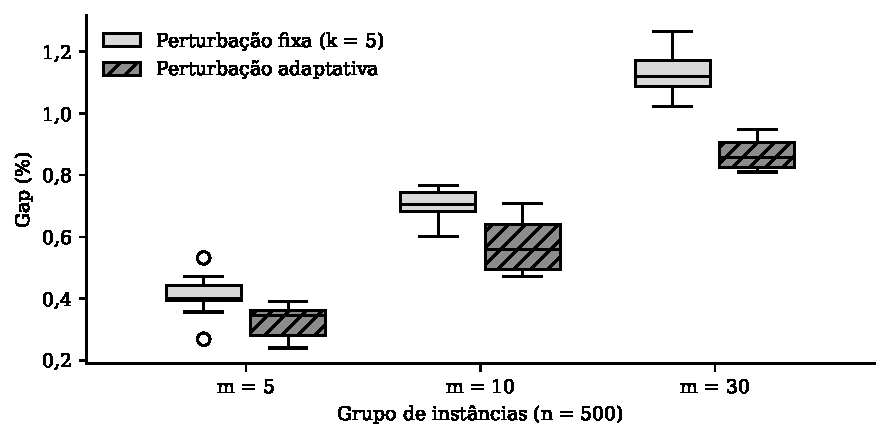
\includegraphics[width=0.85\textwidth]{figuras/cientifico/boxplot-ablacao.pdf}
  \fonteautor
\end{figure}

% ------------------------------------------------------------------------------
\section{Discussão}
\label{sec:experimentos:discussao}

Os resultados respondem afirmativamente à questão de pesquisa apresentada na
\cref{sec:introducao:problema}. Com 60 segundos, a heurística obteve soluções
mais próximas das melhores conhecidas do que o HiGHS em instâncias com 250 e
500 itens. Nas instâncias pequenas, o solucionador continua sendo a melhor
opção. Uma estratégia prática seria usá-lo quando o número de itens for
pequeno e recorrer à heurística nos demais casos.

Em relação ao \acs{ag} de \textcite{chu1998genetic}, a heurística obteve
resultados melhores com menos parâmetros. Os resultados, porém, ainda ficam
abaixo dos métodos híbridos, como o de \textcite{vasquez2001hybrid}, que
usam tempos de execução muito maiores.

Alguns fatores limitam a validade das conclusões. Os resultados do \acs{ag}
foram obtidos da literatura, em hardware diferente. Por isso, a comparação de
tempos entre os dois métodos é apenas aproximada. Além disso, os parâmetros da
heurística foram calibrados nas mesmas classes de instâncias usadas na
avaliação, ainda que com instâncias diferentes, o que pode favorecer o método
proposto nessas classes.

\begin{instrucao}
\orientacao{Ameaças à validade}
Discutir as limitações dos experimentos não enfraquece o trabalho. Pelo
contrário, mostra maturidade científica e antecipa perguntas da banca. Pense
em vieses nos dados, em comparações desiguais (hardware, tempo, implementação)
e em quanto os resultados podem ser generalizados para outros cenários.
\end{instrucao}

% ==============================================================================
% Capítulo 6: Conclusão
% ==============================================================================
\chapter{Conclusão}
\label{cap:conclusao}

\begin{instrucao}
\orientacao{O que vai na Conclusão}
A Conclusão fecha o trabalho. Ela retoma a questão de pesquisa e os objetivos,
mostra como cada um foi atingido, resume as contribuições, reconhece as
limitações e aponta trabalhos futuros. Como referência, de duas a quatro
páginas costumam ser suficientes.

Não apresente resultados novos nem repita a discussão do capítulo anterior. A
Conclusão costuma ter poucas citações, porque trata do que o próprio trabalho
produziu. Uma forma eficaz de organizá-la é percorrer os objetivos
específicos na mesma ordem em que aparecem na Introdução, indicando onde cada
um foi tratado.
\end{instrucao}

Este trabalho propôs uma heurística de \acs{ils} para o \acs{mkp} com
perturbação adaptativa e avaliou seu desempenho em instâncias de referência da
literatura. Os resultados mostraram que, com 60 segundos de execução, a
heurística obtém soluções mais próximas das melhores conhecidas do que o
solucionador HiGHS nas instâncias com 250 e 500 itens, respondendo
afirmativamente à questão de pesquisa formulada na
\cref{sec:introducao:problema}.

Os objetivos específicos foram atingidos da seguinte forma. A revisão das
abordagens heurísticas e das instâncias de referência foi apresentada no
\cref{cap:relacionados}. A heurística proposta e o modelo de \acs{pli} foram
descritos e implementados conforme o \cref{cap:metodologia}. A comparação com
o solucionador e com o \acs{ag} da literatura, bem como a avaliação da
perturbação adaptativa, foram apresentadas no \cref{cap:experimentos}.

% ------------------------------------------------------------------------------
\section{Contribuições e limitações}
\label{sec:conclusao:contribuicoes}

A principal contribuição do trabalho é uma heurística simples, com apenas dois
parâmetros e sem resolver programas lineares durante a busca, que obtém
resultados competitivos em tempo limitado. A análise dos componentes mostrou
que a perturbação adaptativa é responsável por boa parte do ganho de
desempenho, sobretudo nas instâncias com mais restrições.

Como limitações, a heurística ainda fica atrás dos melhores métodos híbridos
da literatura quando o tempo de execução não é restrito. Além disso, a
comparação com o \acs{ag} usou resultados publicados, obtidos em outro
hardware, e a avaliação se restringiu às instâncias da OR-Library.

% ------------------------------------------------------------------------------
\section{Trabalhos futuros}
\label{sec:conclusao:futuros}

\begin{instrucao}
\orientacao{Trabalhos futuros}
Evite listas genéricas como ``melhorar o desempenho'' ou ``testar com mais
dados''. Para cada sugestão, explique por que ela é promissora e como poderia
ser realizada, com base no que o trabalho mostrou.
\end{instrucao}

Os resultados sugerem três direções de continuidade. A primeira é usar a
relaxação linear apenas na construção da solução inicial, o que poderia
aproximar a heurística dos métodos híbridos sem aumentar o custo de cada
iteração. A segunda é adaptar a heurística a variantes do problema com
restrições adicionais, como conflitos entre itens, aproveitando o fato de que
a busca local mantém a viabilidade a cada movimento. A terceira é avaliar a
heurística em instâncias maiores e mais recentes, para verificar se a
vantagem sobre o solucionador se mantém com o crescimento do número de itens.


% ------------------------------------------------------------------------------
% Elementos pós-textuais
% ------------------------------------------------------------------------------
\postextual

% Referências (NBR 6023), geradas pelo Biber a partir de referencias.bib.
\printbibliography[heading=bibintoc]

% Apêndices: material elaborado pelo próprio autor.
\begin{apendicesenv}
% ==============================================================================
% Apêndice A: Declaração de uso de inteligência artificial
% Exigida pelo Art. 19 da Portaria Normativa nº 310/2026 da Ufes.
% Se você não usou ferramentas de IA, apague este arquivo, a linha que o
% inclui no arquivo principal e a Seção 4.3 da Metodologia.
% ==============================================================================
\chapter{Declaração de uso de inteligência artificial}
\label{ap:ia}

\begin{instrucao}
\orientacao{Por que um apêndice?}
O Art. 19 da Portaria Normativa nº 310/2026 da Ufes \cite{ufes2026portaria}
admite que a declaração fique em seção ou apêndice específico. O apêndice foi
escolhido porque a NBR 14724 não prevê um elemento pré-textual para esse fim e
porque o detalhamento das interações exigido pelo § 2º pode ser longo. Por ser
o primeiro apêndice, ele aparece logo após as Referências e é fácil de
localizar. Na Metodologia, uma seção curta cita a ferramenta e remete a este
apêndice.

\orientacao{Como preencher}
\begin{itemize}
  \item No \cref{qua:ia:declaracao}, liste cada ferramenta usada, com a versão
        ou o modelo, a finalidade e a forma de contribuição, indicando as
        partes do trabalho afetadas.
  \item Na seção seguinte, detalhe as interações, informando o que foi pedido,
        por que, como o resultado foi verificado e o que foi aproveitado ou
        descartado.
        Não é preciso transcrever todas as conversas. Descreva os tipos de
        interação com exemplos representativos.
  \item Cite cada ferramenta e inclua-a no arquivo \verb|referencias.bib|
        (veja as entradas \verb|openai2026chatgpt| e \verb|github2026copilot|).
  \item A declaração é escrita na primeira pessoa do singular (``Declaro
        que\ldots''), por ser um compromisso pessoal do autor. O detalhamento
        das interações volta à terceira pessoa, como o restante do trabalho.
  \item Seja específico e honesto. Usos ``meramente acessórios'', que a
        portaria dispensa de declaração, serão definidos pela CPGIA. Na dúvida,
        declare.
\end{itemize}
Substitua o texto de exemplo abaixo pelas ferramentas, versões e usos reais
do seu trabalho. Quando a CPGIA publicar o modelo oficial de declaração,
adapte este apêndice a ele.
\end{instrucao}

% ------------------------------------------------------------------------------
\section{Declaração}

Declaro, em cumprimento ao Art. 19 da Portaria Normativa nº 310/2026 da
\imprimiruniversidade{} \cite{ufes2026portaria}, que utilizei ferramentas de
\acl{ia} na elaboração deste trabalho, nos termos descritos no
\cref{qua:ia:declaracao}. Declaro também que revisei todo o conteúdo gerado
com o auxílio dessas ferramentas, que assumo integral responsabilidade pela
precisão e pela originalidade do texto, do código e dos resultados
apresentados e que nenhuma ferramenta foi tratada como autora ou coautora do
trabalho.

\begin{quadro}[htbp]
  \centering
  \caption{Ferramentas de \acs{ia} utilizadas no trabalho}
  \label{qua:ia:declaracao}
  \small
  \begin{tabularx}{\textwidth}{|>{\raggedright\arraybackslash}p{2.6cm}|>{\raggedright\arraybackslash}X|>{\raggedright\arraybackslash}X|>{\raggedright\arraybackslash}p{2.6cm}|}
    \hline
    \textbf{Ferramenta e versão} & \textbf{Finalidade} &
      \textbf{Forma de contribuição} & \textbf{Partes afetadas} \\
    \hline
    ChatGPT, modelo GPT-5 \cite{openai2026chatgpt} &
      Revisão de redação &
      Sugestões de reescrita de parágrafos já escritos pelo autor, aceitas
      parcialmente após revisão &
      \Cref{cap:introducao,cap:relacionados} \\
    \hline
    ChatGPT, modelo GPT-5 \cite{openai2026chatgpt} &
      Apoio aos testes do código &
      Sugestão de casos de teste para a rotina de verificação de viabilidade,
      implementados e conferidos pelo autor &
      \Cref{sec:metodologia:experimentos} \\
    \hline
  \end{tabularx}
  \fonteautor
\end{quadro}

% ------------------------------------------------------------------------------
\section{Detalhamento das interações}

\textbf{Revisão de redação.} Após escrever a primeira versão da Introdução e
dos Trabalhos Relacionados, o autor submeteu parágrafos isolados à ferramenta,
com pedidos como ``aponte frases ambíguas ou repetitivas neste parágrafo, sem
alterar o conteúdo técnico''. A motivação foi tornar o texto mais claro. As
sugestões foram comparadas com o original. Apenas as que preservavam o sentido
foram incorporadas, com ajustes. Nenhum trecho novo foi gerado pela ferramenta
e nenhuma referência bibliográfica foi obtida por meio dela.

\textbf{Casos de teste.} Durante a implementação, o autor descreveu a função
que verifica a viabilidade de uma solução e pediu sugestões de casos-limite
(mochila vazia, item com peso igual à capacidade, instância com uma única
restrição). Os casos sugeridos foram implementados manualmente como testes
automatizados e executados contra soluções verificadas por outro meio. A
ferramenta não teve acesso ao código-fonte completo, às instâncias nem aos
resultados dos experimentos.

\textbf{Configuração.} As interações ocorreram na interface web da ferramenta,
com as configurações padrão, entre março e outubro de 2026. Nenhum dado
pessoal, sensível ou institucional confidencial foi fornecido.

% ==============================================================================
% Apêndice B: Resultados detalhados
% ==============================================================================
\chapter{Resultados detalhados por grupo de instâncias}
\label{ap:resultados}

\begin{instrucao}
\orientacao{Apêndices e tabelas longas}
Apêndices reúnem material elaborado pelo próprio autor que complementa o texto,
mas que atrapalharia a leitura se ficasse no corpo do trabalho, como
resultados completos, questionários, documentos de requisitos e manuais. Cada apêndice
deve ser citado no texto pelo menos uma vez. Material de outros autores vai em
anexo, e não em apêndice.

Pela NBR 14724:2024, se um apêndice citar obras, as referências dessas obras
ficam no próprio apêndice, e não na lista geral de Referências.

Tabelas que ocupam mais de uma página usam o ambiente \verb|longtable|. O
cabeçalho é repetido no início de cada página, com as indicações
``continua'' e ``continuação'' recomendadas pelo IBGE, como mostra a
\cref{tab:resultados:detalhados}.
\end{instrucao}

A \cref{tab:resultados:detalhados} apresenta o \emph{gap} médio de cada
método em cada um dos 27 grupos de instâncias de \textcite{chu1998genetic},
identificados pelo número de itens ($n$), pelo número de restrições ($m$) e
pelo fator de folga das restrições ($\alpha$).

{\small
\begin{longtable}{@{}rrrrrrr@{}}
  \caption{\emph{Gap} médio (\%) por grupo de instâncias}
  \label{tab:resultados:detalhados} \\
  \toprule
  & & & & & \multicolumn{2}{c}{\acs{ils} proposta} \\
  \cmidrule(l){6-7}
  $n$ & $m$ & $\alpha$ & HiGHS & \acs{ag} & Média & Melhor \\
  \midrule
  \endfirsthead
  \multicolumn{7}{r}{\footnotesize(continuação)} \\
  \toprule
  & & & & & \multicolumn{2}{c}{\acs{ils} proposta} \\
  \cmidrule(l){6-7}
  $n$ & $m$ & $\alpha$ & HiGHS & \acs{ag} & Média & Melhor \\
  \midrule
  \endhead
  \midrule
  \multicolumn{7}{r}{\footnotesize(continua)} \\
  \endfoot
  \bottomrule
  \endlastfoot
    100 & 5 & 0,25 & 0,10 & 0,39 & 0,16 & 0,08 \\
    100 & 5 & 0,50 & 0,06 & 0,27 & 0,11 & 0,05 \\
    100 & 5 & 0,75 & 0,02 & 0,10 & 0,04 & 0,02 \\
    100 & 10 & 0,25 & 0,17 & 0,81 & 0,37 & 0,13 \\
    100 & 10 & 0,50 & 0,14 & 0,58 & 0,26 & 0,12 \\
    100 & 10 & 0,75 & 0,10 & 0,48 & 0,23 & 0,09 \\
    100 & 30 & 0,25 & 0,28 & 1,26 & 0,57 & 0,21 \\
    100 & 30 & 0,50 & 0,27 & 0,88 & 0,48 & 0,22 \\
    100 & 30 & 0,75 & 0,21 & 0,81 & 0,30 & 0,16 \\
    \midrule
    250 & 5 & 0,25 & 0,96 & 0,28 & 0,24 & 0,12 \\
    250 & 5 & 0,50 & 0,64 & 0,22 & 0,16 & 0,08 \\
    250 & 5 & 0,75 & 0,21 & 0,08 & 0,06 & 0,03 \\
    250 & 10 & 0,25 & 1,83 & 0,60 & 0,51 & 0,30 \\
    250 & 10 & 0,50 & 1,50 & 0,61 & 0,44 & 0,24 \\
    250 & 10 & 0,75 & 1,12 & 0,41 & 0,27 & 0,14 \\
    250 & 30 & 0,25 & 2,40 & 0,83 & 0,72 & 0,37 \\
    250 & 30 & 0,50 & 2,39 & 0,82 & 0,58 & 0,37 \\
    250 & 30 & 0,75 & 2,27 & 0,74 & 0,53 & 0,24 \\
    \midrule
    500 & 5 & 0,25 & 2,43 & 0,45 & 0,37 & 0,17 \\
    500 & 5 & 0,50 & 1,55 & 0,29 & 0,24 & 0,13 \\
    500 & 5 & 0,75 & 0,66 & 0,10 & 0,08 & 0,05 \\
    500 & 10 & 0,25 & 5,23 & 0,87 & 0,79 & 0,42 \\
    500 & 10 & 0,50 & 3,79 & 0,63 & 0,57 & 0,40 \\
    500 & 10 & 0,75 & 2,83 & 0,53 & 0,46 & 0,23 \\
    500 & 30 & 0,25 & 7,06 & 1,25 & 0,92 & 0,57 \\
    500 & 30 & 0,50 & 7,22 & 1,26 & 0,95 & 0,54 \\
    500 & 30 & 0,75 & 5,05 & 1,01 & 0,66 & 0,46 \\
\end{longtable}
}
\fonte{Elaborado pelo próprio autor. Os valores do \acs{ag} foram obtidos de
  \textcite{chu1998genetic}.}

\end{apendicesenv}

% Anexos: material de outros autores (por exemplo, um documento de terceiros
% que o trabalho analisa). Descomente e crie o arquivo se precisar.
% \begin{anexosenv}
% \input{cientifico/anexos/a-nome-do-anexo}
% \end{anexosenv}

\end{document}
